\documentclass[12pt, a4paper]{book}%, oneside

\usepackage[headings]{fullpage}
\usepackage{setspace}

% \usepackage[top=1.5cm,right=1.5cm,bottom=1.5cm,left=1.5cm]{geometry}
% \usepackage{fancyhdr}
% \setlength{\headheight}{20pt} 
% \usepackage{graphics}
\usepackage{graphicx}
\usepackage{float}
\usepackage{subfig}
\usepackage{array}
% \usepackage{xtab}
\usepackage{multirow}
\usepackage{booktabs}
\usepackage{longtable}
\usepackage{appendix}
\usepackage[pdfborder={0 0 0}, colorlinks=true, linkcolor=black, citecolor=blue]{hyperref}
\usepackage[printonlyused]{acronym}
\usepackage{algorithmic}
\usepackage{algorithm}
\usepackage{ifpdf}
% ADDED (v0.1): needed for the equations in Chapter 2.
\usepackage{amsmath,amssymb}
% Original diagrams in Chapters 4, 5 and 7 are drawn with TikZ (part of every TeX Live / Overleaf install).
\usepackage{tikz}
\usetikzlibrary{positioning,arrows.meta,fit}
% \setlength{\parindent}{0pt}

% ---------------------------------------------------------------
% Title-page metadata (WORKING DRAFT, research status 16 Nov 2026). Items in [brackets] are NOT confirmed.
% See docs/registers/OPEN_QUESTIONS.md and docs/reports/OPEN_ISSUES_v0.4.md before producing any final title page.
% ---------------------------------------------------------------
\newcommand{\submissionDay}{15}      % NOT CONFIRMED (proposal deadline 5 Jan 2027 is not the submission date)
\newcommand{\submissionMonth}{January}
\newcommand{\submissionYear}{2027}
\newcommand{\submissionDate}{\submissionDay~\submissionMonth,~\submissionYear}
\newcommand{\typeOfThesis}{Bachelor Thesis}

\newcommand{\titleOfThesisOne}{Biologically Plausible Secure Multi-Party Computation for Efficient Privacy-Preserving AI Training I}

% Name as printed on the approved proposal; ID taken from the PDF file name only.
% Deliberately NOT changed. Project records also contain "Abdelmonem Sayed Somida" and the folder
% name "13006494 - Abdelmonem Sayed"; confirm the registered name from the GIU record (docs/reports/OPEN_ISSUES_v0.4.md).
\newcommand{\authorOfThesis}{Abdelmonem Elsayed}
\newcommand{\supervisorOne}{Dr. Nada Sharaf}
\newcommand{\supervisorTwo}{Dr. Mayar Elfares}
\newcommand{\supervisorThree}{}      % unused: no third supervisor confirmed

% Marker for text that needs the student's confirmation or later evidence.
\newcommand{\pending}[1]{\textbf{[#1]}}

% FIX (v0.1): the original macros pointed to images/, which does not exist in the project;
% the only asset directory is figures/. (The macros were unused in the original template.)
\newcommand{\includefig}[4]{
    \begin{figure}[ht]
     \centering
      \includegraphics[width=#1\textwidth]{figures/#2}
      \caption{#3}
      \label{#4}
    \end{figure}
}

\newcommand{\includefigWSC}[5]{
    \begin{figure}[ht]
     \centering
      \includegraphics[width=#1\textwidth]{figures/#2}
      \caption[#3]{#4}
      \label{#5}
    \end{figure}
}

\newcommand{\includeeps}[4]{
\includefig{#1}{#2.eps}{#3}{#4}
}

\newcommand{\includeepsWSC}[5]{
\includefigWSC{#1}{#2.eps}{#3}{#4}{#5}
}

% v0.3: PDF metadata set once via hyperref (duplicate \pdfinfo removed). Author field intentionally left unset until the registered name is confirmed.
\hypersetup{pdftitle={\titleOfThesisOne}, pdfsubject={\typeOfThesis\space -- working draft (research status 16 November 2026)}}

\begin{document}
% \overfullrule=5pt
\pagestyle{plain}
\pagenumbering{Roman}

% Title page (single page). The GIU sample template printed the same page twice with a blank page
% between; that duplication is treated as accidental and removed.
% NOTE: spacing is done with \par / \vspace only (no "\\[..]" tricks).
\newcommand{\titlePage}{%
\thispagestyle{empty}%
\begin{center}
	\vspace*{1cm}
	
\includegraphics[width=3.5cm]{figures/giu_logo.png}\par
	\vspace{5mm}
	{\large\bfseries German International University\par}
	\vspace{2mm}
	{\large\bfseries Faculty of Informatics and Computer Science\par}
	\vspace{2.5cm}
	{\LARGE\bfseries \titleOfThesisOne\par}
	\vspace{2cm}
	{\large\bfseries \typeOfThesis\par}
	\vfill
	\begin{large}
	\begin{tabular}{@{}l@{\hspace{1.5cm}}l@{}}
		Author: & \authorOfThesis \\[3mm]
		Supervisors: & \supervisorOne \\[1mm]
		 & \supervisorTwo \\[3mm]
		Submission Date: & \submissionDate \\
	\end{tabular}
	\end{large}
	\vspace{1.5cm}
\end{center}
\clearpage
}
%++++++++++++++++++++++++++++++++++++++++++++++++++++++++++++++++++++
\titlePage
%++++++++++++++++++++++++++++++++++++++++++++++++++++++++++++++++++++
% Declaration
\thispagestyle{empty}
\null\vspace{3.5cm}
\begin{center}
	{\Large\bfseries Declaration\par}
\end{center}
\vspace{1.5cm}
\begin{center}
\begin{minipage}{0.85\textwidth}
\raggedright
\setlength{\parindent}{0pt}
This is to certify that:

\vspace{6mm}
\begin{list}{}{\setlength{\labelwidth}{1cm}\setlength{\leftmargin}{1.2cm}\setlength{\labelsep}{2mm}\setlength{\itemsep}{5mm}}
\item[(i)] the thesis comprises only my original work toward the Bachelor Degree.
\item[(ii)] due acknowledgement has been made in the text to all other material used.
\end{list}
\end{minipage}
\end{center}

\vspace{3.5cm}
\begin{flushright}
\rule{6cm}{0.4pt}\par
\vspace{2mm}
\authorOfThesis\par
\vspace{1mm}
\submissionDate\par
\end{flushright}
\clearpage


\chapter*{Acknowledgments}
\addcontentsline{toc}{chapter}{Acknowledgments}
\label{chap:ack}
\pending{Student-supplied text only.}


\chapter*{Abstract}
% \addcontentsline{toc}{chapter}{Abstract}
\label{chap:abstract}
% PROVISIONAL abstract describing the state of 16 November 2026. Rewrite after Secure FF results exist.
Secure multi-party computation (MPC) allows several data owners to train a model jointly without revealing their data, but secure training is far more expensive than ordinary training. This thesis asks whether the biologically inspired Forward-Forward (FF) algorithm, which replaces the backward pass of backpropagation (BP) by two forward passes with layer-local objectives, can reduce the computation and communication cost of secure training under a fixed MPC protocol, and whether an MPC-aware modification of FF can reduce its dominant cost further. The study compares four tracks: Plain BP, Secure BP, Plain FF and Secure FF, using MP-SPDZ with the three-party, semi-honest, honest-majority replicated-ring protocol over a 64-bit ring and 16-bit fixed-point precision.

In a plaintext benchmark on a 5,000/1,000/1,000 MNIST split, BP reached $75.96\pm2.89\%$ and FF $59.76\pm3.18\%$ test accuracy over five seeds, with FF using twice as many optimizer updates. Secure BP was developed from bounded scalar prototypes to a batched-matrix program, which reduced the compiled round count by more than three orders of magnitude. One full-size Secure BP run (784--128--128--10, seed 42) completed on a single host in 933 seconds of MP-SPDZ time with 5.2 GB of global communication and reached 77.2\% test accuracy; its losses agree with the matching plaintext run within $4.4\times10^{-4}$. Secure FF has not yet been implemented, so the main research question remains open.

\pending{Provisional abstract for working version 0.4 (research status 16 November 2026). To be rewritten after Secure FF, profiling and the final comparison are complete.}

\tableofcontents
% \addcontentsline{toc}{chapter}{Contents}
\clearpage 

\pagestyle{headings}
\pagenumbering{arabic}

% \setlength\parskip{15pt}
\setlength\parskip{.5\baselineskip plus .2\baselineskip
	minus .4\baselineskip}

\chapter{Introduction}
\label{chap:intro}

\section{Background and Motivation}\label{sec:intro-motivation}
Machine learning increasingly relies on large datasets that are often held by different organisations and are sensitive, for example in healthcare and finance. Pooling the raw records may be undesirable or not permitted. \ac{ppml} aims to allow collaborative computation and learning while limiting the exposure of such data. \ac{mpc} is one cryptographic route to this goal: several parties jointly evaluate a function on their private inputs so that, under the assumptions of a stated security model, no party learns more than the outputs it is entitled to \cite{zhou2024smpc,keller2020mpspdz}.

The practical difficulty addressed in this thesis is cost. Secure training replaces ordinary arithmetic by secret-shared arithmetic that requires interaction between the parties, and operations such as comparison, truncation, exponentiation and division are considerably more expensive than additions and multiplications \cite{keller2022sqt,zhang2025efficient}. Existing efficiency work mostly keeps the learning algorithm fixed and improves the secure-computation stack \cite{yang2025esmpc,wagh2021falcon,keller2022sqt,tan2021cryptgpu,lu2024clover}. The learning algorithm, however, determines which operations must be evaluated securely and which intermediate values must be kept. This motivates the question of whether the learning rule can be co-designed with \ac{mpc} instead of applying \ac{mpc} to \ac{bp} unchanged.

\section{Research Problem}\label{sec:intro-problem}
The thesis studies the \ac{ff} algorithm \cite{hinton2022ff} as the primary alternative learning mechanism. \ac{ff} replaces the forward and backward passes of \ac{bp} by two forward passes, one on positive and one on negative data, and trains every layer with its own local objective. Whether this locality lowers the cost of secure training is not known: possible savings (no backward pass through the network) compete with possible additional costs (two forward passes, secure negative-data generation, per-layer normalisation, a non-linear local loss and a more expensive inference procedure). Speedups of \ac{ff} reported for non-cryptographic distributed training \cite{aktemur2025pff} do not settle the question for \ac{mpc}. The central hypothesis of the project, that co-designing the learning rule and the privacy mechanism can improve the efficiency of privacy-preserving collaborative training, is therefore treated as a hypothesis to be tested and not as an assumption.

\section{Research Questions}\label{sec:intro-rq}
The main research question, as worded in the approved project proposal, is:

\begin{quote}
Under a fixed \ac{mpc} protocol and threat model, how does Forward-Forward training compare with conventional backpropagation-based training in computation cost, communication cost, and model utility, and can an \ac{mpc}-aware modification of \ac{ff} reduce its dominant secure-computation cost at acceptable utility?
\end{quote}

It is refined into three sub-questions.
\begin{description}
  \item[RQ1 (comparison)] How do secure \ac{ff} and secure \ac{bp} compare in training time, communication volume, communication rounds (where measurable) and accuracy at matched settings?
  \item[RQ2 (bottlenecks)] Which secure operations dominate the cost of each method?
  \item[RQ3 (co-design)] Does a bottleneck-motivated modification of the \ac{ff} computation reduce that cost, and at what utility cost?
\end{description}
To answer them, the study is organised around four experimental tracks: \emph{Plain BP}, \emph{Secure BP}, \emph{Plain FF} and \emph{Secure FF}. The plaintext tracks fix the learning behaviour of each algorithm without cryptography; the secure tracks measure the same algorithms under one \ac{mpc} configuration.

\section{Objectives and Current Status}\label{sec:intro-status}
The objectives derived from the research questions are: (O1) establish plaintext baselines for \ac{bp} and \ac{ff} on a common data split; (O2) implement and validate secure \ac{bp} training in MP-SPDZ under a fixed three-party protocol; (O3) implement secure \ac{ff} under the same configuration; (O4) compare the secure methods in cost and utility with repeated runs; (O5) profile the dominant secure operations of both methods; and (O6) design and evaluate one \ac{mpc}-aware modification of \ac{ff} with an ablation.

This document is a working version that records the state of the project on 16 November 2026. Objective O1 is met: Plain BP and Plain FF have been benchmarked over five seeds. Objective O2 is met for one seed: after a series of bounded development runs on a 784--8--10 network, a batched-matrix secure \ac{bp} program trained the full 784--128--128--10 network on the 5{,}000/1{,}000/1{,}000 MNIST split under the three-party replicated-ring protocol, and its seed-42 results agree closely with the recorded Plain BP run for the same seed. Objectives O3--O6 have not started; in particular, \emph{Secure FF has not been implemented or executed}, so RQ1 is only partially addressed and RQ2 and RQ3 remain open.

\section{Contributions}\label{sec:intro-contrib}
The work completed so far contributes:
\begin{enumerate}
  \item a standardised plaintext benchmark of \ac{bp} and \ac{ff} on a common MNIST split with five seeds and documented update and presentation budgets (Chapter~\ref{chap:results});
  \item an end-to-end secure \ac{bp} training implementation in MP-SPDZ, developed from bounded scalar prototypes to a batched-matrix program that trains a 118{,}282-parameter network on 5{,}000 examples in a single three-party execution (Chapter~\ref{chap:impl});
  \item a hash-verified, single-seed measurement of the utility, runtime, communication and memory of that secure run, together with a paired numerical comparison against the matching plaintext run (Chapter~\ref{chap:results}); and
  \item an evidence record (program and input hashes, input-stream verification, separated measurement scopes and an explicit list of unresolved technical issues) on which the remaining Secure FF work can build.
\end{enumerate}
The intended contributions that remain open are a controlled secure \ac{ff}-versus-\ac{bp} comparison under the same \ac{mpc} configuration, a per-operation cost analysis of both methods, and one evidence-driven \ac{mpc}-aware modification of \ac{ff} with an ablation. Evidence that \ac{ff} offers no advantage under \ac{mpc} would be a valid outcome.

\section{Scope and Limitations}\label{sec:intro-scope}
The thesis does not propose a new cryptographic protocol or security model. Every security statement refers only to the protocol and threat model fixed for the experiments: three parties, a semi-honest adversary and an honest majority. All secure runs so far were executed as three party processes on one host, so they measure the cost of the protocol on that host and not the latency of a distributed deployment. The full-size secure result comes from one seed. Conclusions apply to the evaluated configuration (small fully connected networks on MNIST, one protocol, one host). Optional extensions of the proposal (\acp{snn}, selective activation, further datasets and protocols) are outside the core scope and are mentioned only where they are relevant to the literature.

\section{Thesis Organisation}\label{sec:intro-org}
Chapter~\ref{chap:background} introduces the concepts needed for the project. Chapter~\ref{chap:litreview} reviews the related literature and states the preliminary research gap. Chapter~\ref{chap:method} describes the experimental design, the four experimental tracks and the comparisons made between them. Chapter~\ref{chap:impl} describes the implementation, including the bounded and the full-size secure \ac{bp} programs. Chapter~\ref{chap:setup} lists the experimental configurations and measurement definitions. Chapter~\ref{chap:results} reports the plaintext baselines, the bounded secure \ac{bp} runs and the full-size secure \ac{bp} run, and Chapter~\ref{chap:discussion} interprets them and states their limitations. Chapter~\ref{chap:concl} gives an interim conclusion and the remaining work.

\chapter{Background}\label{chap:background}

\begin{sloppypar}
This chapter introduces the concepts needed to follow the rest of the thesis: the privacy-preserving setting, \ac{mpc} and its security models, replicated secret sharing, fixed-point arithmetic and truncation, the two learning algorithms that are compared (\ac{bp} and \ac{ff}), the secure operations they induce, and the way cost is measured. Statements that come from the literature are cited. Statements about the implementation used in this project refer to MP-SPDZ v0.4.4.
\end{sloppypar}

\section{Privacy-Preserving Machine Learning}\label{sec:bg-ppml}
\ac{ppml} denotes techniques that allow models to be trained or evaluated while limiting what is revealed about the underlying data. Surveys describe secure machine learning as built mainly on homomorphic encryption and secret sharing, with different trade-offs between computation, communication, security assumptions and deployment model \cite{zhou2024smpc}. Several paradigms are related but address different threats, and results for one do not transfer automatically to another (Table~\ref{tab:bg-paradigms}).

\begin{table}[ht]
\centering
\small
\begin{tabular}{@{}>{\raggedright\arraybackslash}p{2.6cm}>{\raggedright\arraybackslash}p{5.4cm}>{\raggedright\arraybackslash}p{6.2cm}@{}}
\toprule
Paradigm & What it provides & What it does not provide by itself \\
\midrule
\ac{mpc} & Joint computation of a function over private inputs; under the stated model, parties learn only the intended outputs & Protection against what the released outputs reveal (e.g.\ membership or inversion attacks on a published model) \\
\ac{fhe} / \ac{he} & Computation on ciphertexts, typically performed by one party on data encrypted by another & The interactive, share-based mechanism of \ac{mpc}; costs and trust assumptions differ \\
\ac{fl} & Training data stay local; model updates are exchanged & A cryptographic guarantee: exchanged updates can leak information unless combined with other mechanisms \\
\ac{dp} & A statistical bound on what a released output reveals about any individual record & Protection of inputs during the computation; it must be combined with \ac{mpc} for that \\
\bottomrule
\end{tabular}
\caption{Related privacy paradigms and how they are kept apart in this thesis (definitions after \cite{zhou2024smpc,das2025dpmpc}).}
\label{tab:bg-paradigms}
\end{table}

These mechanisms can be combined; for example, a protocol can train with \ac{dp} noise inside an \ac{mpc} computation \cite{das2025dpmpc}. This thesis keeps five questions conceptually separate: the cryptographic guarantee of the protocol, the leakage permitted by what is finally released, model utility, computation cost and communication cost.

\section{Secure Multi-Party Computation}\label{sec:bg-mpc}
In \ac{mpc}, $n$ parties $P_1,\dots,P_n$ hold private inputs $x_1,\dots,x_n$ and want to compute $y=f(x_1,\dots,x_n)$ so that each party learns $y$ (or its designated part of it) and nothing else about the other inputs, beyond what $y$ itself implies. Security is usually defined by comparison with an ideal world in which a trusted party computes $f$: a protocol is secure if anything an adversary can learn in the real execution could also be simulated from its inputs and outputs alone. Two consequences matter for this project. First, the guarantee always holds relative to a specific protocol, adversary model and number of parties. Second, the output of the computation is not protected: if the trained model is released, the leakage it permits is a separate problem from the input privacy of \ac{mpc} \cite{wagh2021falcon}.

Practical frameworks make \ac{mpc} usable for machine-learning workloads. MP-SPDZ offers one high-level interface, compiler and virtual machine for many protocol variants, so that the same computation can be run under different security models \cite{keller2020mpspdz}. CrypTen provides a PyTorch-like interface with automatic differentiation \cite{knott2021crypten}. This project uses MP-SPDZ.

\section{Security Models and Threat Assumptions}\label{sec:bg-security}
Security models differ along two independent axes \cite{keller2020mpspdz,zhou2024smpc}.

\paragraph{Adversary behaviour.} A \emph{semi-honest} (passive) adversary follows the protocol but tries to learn from the messages it sees. A \emph{malicious} (active) adversary may deviate arbitrarily. Protocols with malicious security differ in what they guarantee when deviation is detected: security with abort stops the computation, whereas \ac{god} ensures that honest parties still receive the output \cite{koti2021swift}.

\paragraph{Corruption threshold.} An \emph{honest-majority} setting assumes fewer than half of the parties are corrupted (for three parties: at most one); a \emph{dishonest-majority} setting allows more. Dishonest-majority protocols generally rely on heavier cryptographic machinery, whereas honest-majority protocols can be considerably cheaper \cite{keller2020mpspdz}. The threat model therefore strongly affects cost, and cost figures from different models are not comparable.

The experiments of this thesis use one configuration: three parties, semi-honest adversary, honest majority (at most one passively corrupted party), as provided by the replicated-ring protocol of MP-SPDZ (referred to as \emph{Rep3 Ring} in this thesis). This is also the main detailed setting of the secure-training experiments of Keller and Sun \cite{keller2022sqt}. Every security statement in the thesis refers only to this configuration. Secure-training systems typically assume static corruption and secure point-to-point channels, and generally leave side-channel and denial-of-service attacks out of scope \cite{yang2025esmpc,wagh2021falcon}.

\section{Secret Sharing and Replicated Sharing}\label{sec:bg-sharing}
\emph{Additive secret sharing} over a ring $\mathbb{Z}_{2^k}$ splits a value $x$ into shares with $x = x_0 + x_1 + x_2 \pmod{2^k}$. Any proper subset of the shares is uniformly distributed and reveals nothing about $x$. Addition of shared values and multiplication by public constants are local operations; multiplication of two shared values requires interaction.

\emph{Replicated secret sharing} (\ac{rss}) for three parties additionally gives party $P_i$ two of the three additive shares, $(x_i, x_{i+1})$ with indices modulo $3$. Each pair of parties therefore jointly holds all shares, while a single party misses one share. This 2-out-of-3 sharing is used by several three-party training systems \cite{wagh2021falcon,tan2021cryptgpu,keller2022sqt}. As an illustration of the principle (not a description of the exact MP-SPDZ implementation), the product $z = xy$ expands into nine cross terms $x_i y_j$, and party $P_i$ can compute locally the three terms
\begin{equation}
  z_i' = x_i y_i + x_i y_{i+1} + x_{i+1} y_i ,
  \label{eq:rss-mult}
\end{equation}
which together cover all nine terms over $i\in\{0,1,2\}$. Re-randomising these partial results with correlated randomness and exchanging them restores a replicated sharing of $z$. The precise message pattern, round count and randomness generation depend on the protocol implementation and are not assumed here. Shamir secret sharing is a different threshold scheme over a finite field or Galois ring, used for example by the protocols of Zhang et al.\ and Zhou \cite{zhang2025efficient,zhou2026rmfe}; it is not the scheme used in this project.

Some systems rely on a trusted party or dealer to generate correlated randomness such as Beaver triples \cite{knott2021crypten,smajlovic2023sequre}. This is an additional assumption and must be stated when results are compared. Protocols are often divided into an input-independent \emph{preprocessing} phase and an \emph{online} phase; the distinction matters for cost measurement (Section~\ref{sec:bg-cost}).

\section{Secure Arithmetic, Fixed-Point Representation and Truncation}\label{sec:bg-fixed}
Secret-shared arithmetic operates on integers modulo $2^k$ (or a prime), whereas neural networks use real numbers. A \emph{fixed-point} encoding with $f$ fractional bits maps a real $x$ to the integer
\begin{equation}
  \tilde{x} = \operatorname{round}\!\left(2^{f}x\right),
  \label{eq:fixed}
\end{equation}
where $\operatorname{round}$ denotes rounding to the nearest integer, so the quantisation step is $2^{-f}$. In MP-SPDZ, \texttt{sfix(f,k)} is such a representation with $f$ fractional bits and $k$ bits in total; the MP-SPDZ documentation describes the default $f=16$, $k=31$ as allowing numbers up to about $2^{k-f-1}=2^{14}=16384$ in magnitude, with a smallest non-zero magnitude of $2^{-16}$. Values outside the representable range wrap around silently; overflow and wrap-around are recognised practical difficulties of \ac{mpc}-based machine learning \cite{knott2021crypten,zhang2025efficient}.

The product of two encoded values carries $2f$ fractional bits and must be \emph{truncated} by $f$ bits to return to the original scale. Exact truncation requires secure bit operations. \emph{Probabilistic truncation} is cheaper: it rounds $a/2^{m}$ randomly down or up, where the probability of rounding up is the discarded fraction $(a \bmod 2^{m})/2^{m}$, so the result is random within a small range around the exact value, provided the operands respect the bit-length assumptions of the construction. MP-SPDZ uses probabilistic truncation by default for fixed-point multiplication and division and offers deterministic rounding to nearest as a more expensive alternative (\texttt{sfix.round\_nearest}), which is not used in this thesis. Keller and Sun use probabilistic truncation in their training protocols and report that lower precision slightly increases error \cite{keller2022sqt}.

The bit-length assumption matters in a ring. In the replicated-ring protocol of MP-SPDZ, a truncation of a $k$-bit value is executed by a cheaper, low-round variant only if $k$ plus a statistical security margin (by default $40$ bits) fits into the ring; otherwise a variant with an additional correction step is used. With a 64-bit ring and $k$ of up to $63$ bits, the margin cannot be met, and the virtual machine reports after the run that the domain is too small for low-round truncation. The consequences of this message for the runs of this project are discussed with the experiments.

Probabilistic truncation also has a security aspect. The MP-SPDZ compiler warns that probabilistic truncation leaks some information and refers to the work of Santos et al.\ \cite{santos2024curl}, whose abstract states that it proves the security of widely used probabilistic-truncation protocols in the stand-alone model. That result is not assumed to extend automatically to every truncation branch of a framework, to the exact variant executed in this project, or to arbitrary composition, so no claim of zero leakage is made in this thesis; the choice is treated as a limitation of the threat-model discussion.

Nonlinear routines such as comparison use, in ring protocols, a local split of each arithmetic share into binary summands (the compiler option \texttt{use\_split}); with value $3$ it refers to a three-way split and not to the number of parties. Floating-point secure training is an alternative representation: BEACON reports secure floating-point training in a two-party semi-honest setting with speedups against the floating-point baselines it tests \cite{rathee2023beacon}. It is not considered further here.

\section{Neural-Network Training Fundamentals}\label{sec:bg-nn}
A \ac{mlp} with $L$ layers computes, for input $\mathbf{a}^{(0)}=\mathbf{x}$,
\begin{align}
  \mathbf{z}^{(l)} &= W^{(l)}\mathbf{a}^{(l-1)} + \mathbf{b}^{(l)}, \quad l=1,\dots,L, \label{eq:mlp-pre}\\
  \mathbf{a}^{(l)} &= \sigma\!\left(\mathbf{z}^{(l)}\right), \quad l=1,\dots,L-1, \label{eq:mlp-hidden}
\end{align}
where $W^{(l)}$ and $\mathbf{b}^{(l)}$ are the weights and biases of layer $l$ and $\sigma$ is the hidden nonlinearity, here the rectified linear unit $\mathrm{ReLU}(z)=\max(0,z)$. The final layer is linear: its pre-activation $\mathbf{z}^{(L)}$ is the vector of logits. For $C$-class classification the probabilities are $p_c = \exp(z^{(L)}_c)/\sum_{j}\exp(z^{(L)}_j)$ and the cross-entropy loss for true class $y$ is $\mathcal{L} = -\log p_y$. Training minimises the average loss by \ac{sgd}: for a mini-batch the parameters $\theta$ are updated as $\theta \leftarrow \theta - \eta\,\nabla_\theta \mathcal{L}$ with learning rate $\eta$. Mini-batches, epochs, learning rate and initialisation are hyperparameters that affect both utility and the number of secure operations.

\section{Backpropagation}\label{sec:bg-bp}
\ac{bp} computes $\nabla_\theta\mathcal{L}$ by applying the chain rule from the output layer to the input layer. With $\boldsymbol{\delta}^{(l)}=\partial\mathcal{L}/\partial\mathbf{z}^{(l)}$ and the convention of Equations~\eqref{eq:mlp-pre}--\eqref{eq:mlp-hidden},
\begin{align}
  \boldsymbol{\delta}^{(L)} &= \mathbf{p} - \mathbf{e}_y, \label{eq:bp-out}\\
  \boldsymbol{\delta}^{(l)} &= \left(W^{(l+1)\top}\boldsymbol{\delta}^{(l+1)}\right)\odot\sigma'\!\left(\mathbf{z}^{(l)}\right), \quad l=L-1,\dots,1, \label{eq:bp-hidden}\\
  \frac{\partial\mathcal{L}}{\partial W^{(l)}} &= \boldsymbol{\delta}^{(l)}\mathbf{a}^{(l-1)\top}, \qquad
  \frac{\partial\mathcal{L}}{\partial \mathbf{b}^{(l)}} = \boldsymbol{\delta}^{(l)}, \quad l=1,\dots,L, \label{eq:bp-grad}
\end{align}
where $\mathbf{e}_y$ is the one-hot vector of the true class and $\odot$ the element-wise product. Equation~\eqref{eq:bp-out} holds only for softmax with cross-entropy and a linear-logit output layer. Two properties are important under \ac{mpc}. First, every layer's update depends on the error signal of the layer above, so the backward pass is a sequential dependency across layers and needs the stored forward quantities. Second, the derivative of ReLU is a step function; the implementation used in this project takes $\sigma'(z)=1$ if $0<z$ and $0$ otherwise (so $\sigma'(0)=0$), which in secret-shared form requires a secure comparison. In a related \ac{mpc} setting, SecP-Tuning removes backward propagation and optimisation from the \ac{mpc} computation for LLM prompt tuning, with a data-owner/server interaction that differs from the setting of this thesis \cite{luo2026secptuning}.

\section{Forward-Forward Learning}\label{sec:bg-ff}
\ac{ff} was proposed by Hinton as a learning procedure motivated by biological plausibility \cite{hinton2022ff}. The global forward-and-backward procedure is replaced by two forward passes: a \emph{positive} pass on real data and a \emph{negative} pass on data that the network should reject. Each layer has its own objective that makes its \emph{goodness} high for positive data and low for negative data. In Hinton's formulation the goodness of layer $l$ is the sum of squared activities,
\begin{equation}
  g^{(l)} = \sum_{j} \left(a^{(l)}_j\right)^2 ,
  \label{eq:goodness}
\end{equation}
and the probability that an input is positive is modelled as $\Pr(\text{pos}) = \mathrm{sigmoid}\!\left(g^{(l)}-\theta\right)$ with a threshold $\theta$. A common local loss is the logistic loss of this quantity, which, written with the softplus function $\mathrm{softplus}(u)=\log(1+e^{u})$, is
\begin{align}
  \ell^{(l)} &= \mathrm{softplus}\!\left(\theta - g^{(l)}\right)\ \text{for positive data}, \label{eq:ff-loss-pos}\\
  \ell^{(l)} &= \mathrm{softplus}\!\left(g^{(l)} - \theta\right)\ \text{for negative data}. \label{eq:ff-loss-neg}
\end{align}
The output of a layer is length-normalised before it is passed on, so that the next layer cannot simply read the previous layer's goodness. In supervised image classification the label is embedded in the input; positive data carry the correct label and negative data a wrong one \cite{hinton2022ff}. At inference, the network is evaluated once per candidate label and the label with the highest accumulated goodness is chosen; variants instead train a classifier on the layer activities.

Three clarifications keep the description accurate. \ac{ff} avoids propagating a global error signal backwards through the whole network but it is \emph{not gradient-free}: each layer's local objective is still minimised with gradient-based updates, and some variants add a classifier trained with backpropagation \cite{aktemur2025pff,chen2025scff}. Hinton describes the investigations as preliminary, reports results on small networks, and leaves large-scale behaviour open \cite{hinton2022ff}. Finally, \ac{ff} has no inherent cost advantage under \ac{mpc}: removing the global backward pass does not by itself reduce secure cost, because the two passes, secure handling of negative data, normalisation, the nonlinear loss and the inference procedure can all add secure computation.

\section{Secure Operations Relevant to BP and FF}\label{sec:bg-ops}
Under \ac{mpc}, linear operations on shares are cheap compared to nonlinear ones. Table~\ref{tab:bg-ops} lists the operations expected in each method and how they are typically realised. It is an inventory of \emph{hypotheses} taken from the approved proposal and the literature, not a measurement; per-operation costs are to be established by profiling.

\begin{table}[ht]
\centering
\small
\begin{tabular}{@{}>{\raggedright\arraybackslash}p{2.4cm}>{\raggedright\arraybackslash}p{3.6cm}>{\raggedright\arraybackslash}p{3.6cm}>{\raggedright\arraybackslash}p{3.5cm}@{}}
\toprule
Step & \ac{bp} & \ac{ff} & Typical secure realisation \\
\midrule
Linear layers & $W\mathbf{a}$ in forward and $W^\top\boldsymbol\delta$ in backward pass & $W\mathbf{a}$ in two forward passes & Share multiplications plus truncation \\
ReLU & Forward value; derivative (step function) in backward pass & Forward value & Secure comparison with zero \\
Objective & Softmax and cross-entropy & Goodness (squares) and sigmoid/softplus of $g-\theta$ & Exponentiation and division, or approximations \cite{keller2022sqt,zhang2025efficient} \\
Normalisation & Optional & Length normalisation between layers & Division or inverse square root \cite{keller2022sqt} \\
Update & Backward products through all layers; stored forward values & Local updates per layer & Share multiplications plus truncation \\
Data handling & Secret-shared labels & Negative data must be generated without revealing true labels & Secure sampling / label handling \\
Inference & One forward pass & One pass per candidate label, or auxiliary classifier & As above \\
\bottomrule
\end{tabular}
\caption{Candidate secure-operation inventory for BP and FF, adapted from the approved project proposal; to be established by profiling.}
\label{tab:bg-ops}
\end{table}

Protocols for several of these nonlinear operations exist. Falcon gives protocols for ReLU, max-pooling, division and batch normalisation in a three-party replicated setting \cite{wagh2021falcon}. Keller and Sun contribute protocols for exponentiation and inverse square root \cite{keller2022sqt}. Zhang et al.\ propose an approximate softmax for Shamir sharing \cite{zhang2025efficient}. Which primitive dominates the cost of \ac{ff} is unknown and is the subject of research question~2.

\section{Matrix Operations in Secure Training}\label{sec:bg-matrix}
How a secure computation is \emph{expressed} strongly affects its cost, even when the mathematical function is the same. A fully connected layer applied to a mini-batch can be written either as many scalar multiply-and-add operations or as one matrix product $Z = XW$, where the rows of $X$ are the examples of the batch and $W$ is stored as an input-by-output matrix. In secret-shared arithmetic, every product of two shared fixed-point values needs interaction and a truncation. A scalar formulation therefore pays for one truncation (and, in a naive schedule, one round of interaction) per product, whereas a matrix formulation can accumulate each output element exactly and truncate it once, and can batch the interaction for the whole product. MP-SPDZ exposes such products for shared matrices; the backward pass of \ac{bp} needs the same kind of products in transposed form, $\boldsymbol{\Delta}^{(l)}W^{(l)\top}$ for the error signal and $A^{(l-1)\top}\boldsymbol{\Delta}^{(l)}$ for the weight gradient. Nonlinear steps (the ReLU comparison, the softmax and the logarithm of the loss) remain element-wise secure operations. Matrix formulation changes the cost of the computation, not the learning rule: a batched-matrix program and a scalar program for the same network compute the same \ac{bp} update up to fixed-point rounding.

\section{Measuring Cost under MPC}\label{sec:bg-cost}
Cost is reported along several dimensions that must not be conflated. \emph{Runtime} can be measured by the framework itself or by an external timer around the command that compiles and launches the parties; the two have different boundaries and are reported separately. Either can include computation, communication, waiting, synchronisation, preprocessing and framework overhead, and a separate pure-computation time is claimed only if it is instrumented. \emph{Online} and \emph{preprocessing} time or communication are distinguished only when the framework reports them separately; the survey of Zhou et al.\ notes that secure preprocessing is often overlooked \cite{zhou2024smpc}. \emph{Global communication volume} is the amount of data sent by all parties together, whereas a per-party figure covers one party only; it must also be stated whether preprocessing is included. Communication volume is not network latency. \emph{Rounds} count sequential interaction steps and matter more under high latency. MP-SPDZ reports two different round figures: the compiler prints a virtual-machine round count, which is a compile-time statistic, and a running party prints an approximate count of its own communication rounds. Neither is a measurement of online network rounds, and the two are not interchangeable. Per-operation costs are reported only if instrumentation exposes them. Frameworks differ in which counters they expose \cite{keller2020mpspdz}, and figures with different measurement boundaries are not comparable.

Which resource dominates depends on the system. ESMPC profiles the bottlenecks of secure training under the Piranha framework and introduces pipeline and communication optimisations for its two- and three-party GPU settings \cite{yang2025esmpc}, whereas Falcon reports that, for large networks over a wide-area network, compute can dominate the cost \cite{wagh2021falcon}. No universal claim about the dominant cost can therefore be made.

\section{Optional Extension: Spiking Neural Networks}\label{sec:bg-snn}
\acp{snn} encode information in discrete spike events over time. A \ac{lif} neuron integrates its input into a membrane potential that decays over time and emits a spike when the potential crosses a threshold \cite{aribe2025snn}. Under \ac{mpc}, the threshold test is a secure comparison, and the temporal dimension multiplies the amount of computation. For \ac{fhe}-based evaluation, SpyKing reports that the cost of the spiking model depends on the temporal sequence length \cite{nikfam2025spyking}. \acp{snn} are an optional extension of the project and are mentioned here only because they appear in the literature reviewed in the next chapter.

\chapter{Literature Review}\label{chap:litreview}

This chapter reviews the literature thematically. Its argument is: secure neural-network training under \ac{mpc} is feasible but costly; the cost depends on the operations, the protocol and the system; \ac{ff} changes the computation graph of learning and has been studied and optimised in non-cryptographic settings; the privacy work on \acp{snn} identified in this review is adjacent (encrypted evaluation or training-data leakage) rather than a secure-\ac{mpc} comparison; and a controlled experimental comparison of \ac{ff} and \ac{bp} under one specified \ac{mpc} configuration is therefore worth testing. This is a \emph{preliminary} gap derived from a non-exhaustive search, not a claim of novelty.

\paragraph{Scope and sources.} The review covers the 23 references of the approved project proposal, all of which were read by the author, and three later additions that are distinguished as supplementary: two works from 2026 (Zhou \cite{zhou2026rmfe}; Elnady et al.\ \cite{elnady2026ff}) and the multi-party training framework of Lu, Basaran and G\"uler \cite{lu2024clover}, whose introduction, problem formulation and experimental section were read for this version. One further entry supports a specific technical statement rather than the thematic review: the probabilistic-truncation analysis of Santos et al.\ \cite{santos2024curl}, characterised from its abstract. The full-text files of six proposal references \cite{keller2023note,luo2026secptuning,yan2025comet,feng2025fwdp,nikfam2025spyking,kim2022privatesnn} are not part of the project archive. The characterisations of these six therefore follow the project's literature records and the official abstracts. Numerical results quoted below always carry the setting of the paper that reports them; they use different protocols, hardware, networks, models and baselines and are not comparable with each other or with the measurements of this thesis.

\section{MPC for Privacy-Preserving Machine Learning}\label{sec:lr-mpc}
The survey by Zhou et al.\ organises secure machine learning by security model, system type and deployment model and discusses secret sharing and homomorphic encryption. In the systems it surveys, secret-sharing approaches often compute faster than homomorphic-encryption approaches but may need more communication; this is a trend in the reviewed work and not a universal law \cite{zhou2024smpc}. It is a survey and does not benchmark \ac{ff}.

Two frameworks matter for the experimental part. MP-SPDZ provides a high-level interface, a compiler and a virtual machine for many \ac{mpc} protocols and security settings, so that a computation can be written once and run under different assumptions \cite{keller2020mpspdz}; it is the implementation framework of this project, and statements about security always have to name the selected protocol. CrypTen offers a PyTorch-like tensor and automatic-differentiation interface under a semi-honest model in which a trusted party can supply correlated randomness; its published evaluations concentrate on private inference rather than on a comprehensive secure-training study \cite{knott2021crypten}.

Neighbouring paradigms must not be confused with \ac{mpc}. Salam et al.\ combine homomorphic encryption with federated collaboration \cite{salam2023mpppml}; this is a different mechanism from secret-sharing \ac{mpc}, and it is mentioned only to illustrate the paradigm. Federated learning on its own does not give a cryptographic guarantee, and \ac{dp} protects released outputs, not inputs during computation.

\section{Secure Training Systems and Baselines}\label{sec:lr-systems}
Keller and Sun build quantised neural-network training on MP-SPDZ and contribute secure protocols for operations such as exponentiation and inverse square root. In their three-party honest-majority experiment a convolutional MNIST network reaches about 99.2\% accuracy in about 3.5 hours; further networks and datasets are also evaluated, and the paper discusses numerical error and the cost of nonlinear operations \cite{keller2022sqt}. A later note by the same authors identifies an implementation error in the max-pooling backward-gradient routing that explains an accuracy gap observed in the earlier work \cite{keller2023note}; it is a correction note and not a claim that quantisation never changes accuracy. This framework is the closest methodological precedent for the present work, although its models are far larger than the bounded prototype used here.

Falcon is a three-party honest-majority framework with semi-honest and malicious (with abort) variants. In its own private-training setup it reports about $6\times$ faster training than SecureNN and $4.4\times$ than ABY3 with $2$--$60\times$ less communication, finds that compute can dominate for large networks in a wide-area setting, and excludes inference attacks on released outputs \cite{wagh2021falcon}. CryptGPU runs secure learning on GPUs in a replicated-sharing setting and reports speedups against specific prior secure baselines; some comparisons depend on batch size and extrapolated training settings \cite{tan2021cryptgpu}. ESMPC targets secure training in two- and three-party semi-honest settings, profiles bottlenecks under the Piranha framework and introduces pipeline and protocol optimisations; against its Piranha-based baseline its abstract reports training-time reductions of over 30\% for AlexNet and over 45\% for FCNN, LeNet and ViT in the two-party setting, and over 45\% for all four models in the three-party setting \cite{yang2025esmpc}. SWIFT provides maliciously secure three-party computation over rings with \ac{god} in an honest-majority setting, plus a four-party extension. It benchmarks logistic-regression training and inference and deep-network \emph{inference} (LeNet, VGG16) in a 64-bit-ring wide-area setting; neural-network training would require mixed-world conversions that the paper leaves as future work \cite{koti2021swift}. The more recent work of Zhou uses Shamir sharing over Galois rings with reverse multiplication-friendly embedding (RMFE) packing and mixed-circuit techniques for comparisons, truncation, activations, pooling and loss computation. It trains fully connected and convolutional networks on MNIST for at least three parties with an honest majority of passively corrupted parties; relative to its Galois-ring packing baseline at equal packing density it reports $71.4$--$75.1\%$ lower communication and $55.3$--$70.1\%$ faster online training in a local-area network, and $5.3$--$68.1\%$ faster in a wide-area network across its three networks, on its own hardware and network settings \cite{zhou2026rmfe}. It shows that secure-training optimisation is still advancing but it does not study \ac{ff}, and its protocol differs from the replicated-ring configuration used here.

Scalability in the number of parties is a separate axis. Lu, Basaran and G\"uler argue that information-theoretic multi-party training frameworks based on Lagrange coded computing suffer from communication that grows quadratically with the number of users, because polynomial degree reduction is needed after every multiplication. Their framework, CLOVER, introduces a degree-reduction mechanism (Double Lagrange Coding) that moves the quadratic part of the communication to a data-independent offline phase and achieves linear communication complexity under information-theoretic privacy against up to $T$ colluding honest-but-curious users \cite{lu2024clover}. It operates over a prime field and, to remain polynomial, trains neural networks with quadratic activations rather than ReLU; its experiments train a one-hidden-layer network with 128 hidden units on MNIST and on VGG features of CIFAR-10 and report, against its COPML baseline, about $28\times$ and $26\times$ lower communication and $6\times$ and $4.8\times$ faster training, respectively, in its own distributed setting \cite{lu2024clover}. The work is relevant here because it treats communication as the scaling bottleneck of multi-party training and because it separates offline from online communication, but it changes the network (polynomial activations) and the sharing scheme, and it does not study \ac{ff}.

Table~\ref{tab:lr-mpc} summarises these works with the setting and the limits that matter for this thesis.

\begin{table}[ht]
\centering
\footnotesize
\begin{tabular}{@{}>{\raggedright\arraybackslash}p{2.2cm}>{\raggedright\arraybackslash}p{3.8cm}>{\raggedright\arraybackslash}p{3.6cm}>{\raggedright\arraybackslash}p{4.0cm}@{}}
\toprule
Work & Setting and security model & Task & Limits for this thesis \\
\midrule
Keller--Sun \cite{keller2022sqt} & MP-SPDZ; three parties, honest majority (main experiment) & Quantised training; MNIST CNN and others & Models far larger than the bounded prototype; not \ac{ff} \\
Falcon \cite{wagh2021falcon} & Three parties; semi-honest and malicious with abort & Private training and inference & Outputs not protected; own network setting \\
CryptGPU \cite{tan2021cryptgpu} & Replicated sharing, GPU & Secure learning & Baseline- and batch-size-dependent speedups \\
ESMPC \cite{yang2025esmpc} & Two and three parties, semi-honest, GPU & Training: FCNN, LeNet, AlexNet, ViT & Gains relative to its Piranha baseline \\
SWIFT \cite{koti2021swift} & Three/four parties, honest majority, malicious, \acs{god} & Logistic-regression training and inference; DNN inference & DNN training left as future work \\
Zhou \cite{zhou2026rmfe} & Shamir over Galois rings, $n\ge3$, semi-honest, $t<n/2$ & Training: fully connected and convolutional MNIST networks & Different sharing scheme and environment; not \ac{ff} \\
CrypTen \cite{knott2021crypten} & Semi-honest; trusted party for randomness & Mainly private inference & Not a comprehensive training study \\
CLOVER \cite{lu2024clover} & Lagrange coded computing over a prime field; $N$ users, up to $T$ honest-but-curious colluders & Training of polynomial (quadratic-activation) networks; MNIST, CIFAR-10 features & Different network and sharing scheme; not \ac{ff} \\
\bottomrule
\end{tabular}
\caption{Secure-training and inference systems relevant to this thesis, as characterised in the cited papers.}
\label{tab:lr-mpc}
\end{table}

\section{Protocol-Level and System Optimisations}\label{sec:lr-opt}
Optimisation work has been carried out at several layers of the stack while keeping the learning algorithm fixed. At the system layer, GPU acceleration \cite{tan2021cryptgpu} and compiler or runtime design \cite{smajlovic2023sequre} reduce time; Sequre targets biomedical secure-computation workloads and relies on an auxiliary trusted dealer for correlated randomness, an additional assumption that must be stated whenever its results are discussed \cite{smajlovic2023sequre}. At the protocol layer, Zhang et al.\ use Shamir sharing and propose secure fixed-point arithmetic, a Winograd-based convolution that reduces the multiplications of one $2\times2$-output, $3\times3$-kernel convolution from 36 to 16, and an approximate softmax; their evaluation concerns protocols and primitives rather than complete training runs \cite{zhang2025efficient}.

Das et al.\ show that the learning procedure and the protocol interact: their two-party protocol combines \ac{mpc} with \ac{dp} and reports $56$--$794\times$ lower communication and $16$--$182\times$ lower runtime than earlier secure-and-private protocols in its selected comparisons, where some baseline runtimes are lower-bound estimates because earlier code was unavailable \cite{das2025dpmpc}. This is a \ac{dp}-\ac{mpc} result and not a speedup of pure \ac{mpc}.

A common observation is that the cost of a secure operation is highly non-uniform and that the learning algorithm determines which operations occur. SecP-Tuning is \ac{mpc}-based forward-only prompt tuning of \acp{llm} with a data-owner/server interaction; it reduces the cost of backward propagation, optimisation and softmax attention in its setting, and its abstract reports roughly $12\times$ and $16\times$ end-to-end acceleration and $17\times$ and $20\times$ lower communication against full-parameter fine-tuning and gradient-based prompt tuning, respectively \cite{luo2026secptuning}. It is not the \ac{ff} algorithm, and its offloading and trust model differ from this thesis. Comet is \ac{mpc}-based private \emph{inference} for \acp{llm}: it predicts activation sparsity, protects the input-dependent sparsity pattern, and reports $1.87$--$2.63\times$ speedup and $1.94$--$2.64\times$ lower communication in its workloads \cite{yan2025comet}. Neither paper evaluates secure training with \ac{ff}.

\section{Fixed-Point and Floating-Point Training}\label{sec:lr-numeric}
The numerical representation affects both accuracy and cost. Keller and Sun develop fixed-point training with probabilistic truncation \cite{keller2022sqt}; CrypTen and Zhang et al.\ discuss overflow, wrap-around and truncation effects \cite{knott2021crypten,zhang2025efficient}. BEACON provides secure floating-point training in a two-party semi-honest setting and reports multi-fold improvements over the floating-point libraries and protocols it compares against; its numbers cannot be read as a general advantage over fixed-point training or over other frameworks \cite{rathee2023beacon}. For \ac{ff}, which uses squared activities, normalisation and a nonlinear loss, ranges and precision are particular concerns; no source reviewed here evaluates them under \ac{mpc}.

\section{Forward-Forward and Local Learning}\label{sec:lr-ff}
Hinton introduces \ac{ff} with positive and negative passes and layer-local goodness objectives. The paper evaluates relatively small networks, finds \ac{ff} competitive in some settings and worse or slower than \ac{bp} in others, and describes the study as preliminary, leaving larger-scale behaviour open \cite{hinton2022ff}. Self-Contrastive \ac{ff} generates positive and negative examples from the data themselves for unsupervised local learning and reports, in its settings, $98.70\pm0.01\%$ on MNIST with a two-hidden-layer perceptron (2{,}000 units per layer), $99.37\pm0.06\%$ with a convolutional network, $80.75\pm0.12\%$ on CIFAR-10 and $77.30\pm0.12\%$ on STL-10; on STL-10 an additional fine-tuning stage uses end-to-end backpropagation, so the extended pipeline is not purely local \cite{chen2025scff}.

Elnady et al.\ compare \ac{ff} with \ac{bp} on six datasets and tune \ac{ff} hyperparameters with two conventional and four metaheuristic methods on four of them, reporting validation-accuracy gains (for example 93\% to 97\% on Pneumonia-MedMNIST and 87\% to 91\% on Fashion-MNIST) together with comparable or reduced training time in their settings \cite{elnady2026ff}. Their \ac{ff} runs use Hinton's implementation while \ac{bp} uses the default training function of a numerical-computing toolbox, so the two methods are not necessarily matched in implementation or computational boundary, and the work involves no cryptography.

Forward-learning methods have also been combined with differential privacy. The method of Feng et al.\ adds noise and privacy guarantees to forward learning, but it is not the \ac{ff} algorithm and it does not use \ac{mpc} \cite{feng2025fwdp}.

\section{Distributed and Federated Forward-Forward}\label{sec:lr-dist}
The layer-wise structure of \ac{ff} has been exploited for parallelism. \ac{pff} distributes layer training over four compute nodes; in one MNIST experiment an all-layers configuration with adaptive negative data reaches $98.51\%$ against $98.52\%$ for the sequential baseline, in $2980.76$\,s against $11190.72$\,s, a $3.75\times$ speedup. It uses no cryptography, and its faster softmax variants add a classifier trained with backpropagation \cite{aktemur2025pff}. A pipeline-parallel speedup does not establish a speedup under \ac{mpc}, because it concerns waiting time between compute nodes and not secure-operation cost. FedFwd integrates \ac{ff}-style local training into federated learning and compares it with backpropagation-based federated methods; its results depend on the data distribution (i.i.d.\ and non-i.i.d.), and it is a workshop paper \cite{park2023fedfwd}. Federated learning alone is not a cryptographic guarantee and is not \ac{mpc}.

\section{Spiking Neural Networks and Privacy}\label{sec:lr-snn}
Aribe reviews surrogate-gradient training, \ac{ann}-to-\ac{snn} conversion and \ac{stdp} and notes that some hardware figures are taken from other literature rather than measured by the author \cite{aribe2025snn}; such figures are not used as evidence of cost under \ac{mpc}. SpyKing uses BFV fully homomorphic encryption, not \ac{mpc}: LeNet5 and a spiking counterpart are trained in a PyTorch phase and then evaluated on encrypted data, and ReLU and other nonlinear operations require decrypting and re-encrypting intermediate values in the described implementation, so the pipeline is not end-to-end encrypted through its nonlinear layers; the cost of the spiking model depends on the temporal sequence length \cite{nikfam2025spyking}. PrivateSNN addresses leakage of training data during conversion from an \ac{ann} and class leakage from the converted parameters, using synthetic samples; within its own setting it reports a performance drop below about 2\% and a large energy-efficiency gain, and it is not a secure-computation protocol \cite{kim2022privatesnn}. \ac{fhe} evaluation of \acp{snn} does not establish \ac{snn} training under \ac{mpc}, and biological inspiration is neither a privacy guarantee nor, on this evidence, automatically cheaper under encryption. This topic is optional for the thesis.

\section{Work at the Intersection of MPC and Biologically Plausible Learning}\label{sec:lr-intersection}
Adjacent work touches the intersection from several sides: SecP-Tuning removes backward computation in \ac{mpc}-based prompt tuning \cite{luo2026secptuning}; Comet exploits activation sparsity for \ac{mpc} inference \cite{yan2025comet}; \ac{ff} has been parallelised and used in federated training without cryptography \cite{aktemur2025pff,park2023fedfwd} and optimised without cryptography \cite{elnady2026ff}; and \acp{snn} have been studied under \ac{fhe} \cite{nikfam2025spyking}. Table~\ref{tab:lr-adjacent} places these side by side.

\begin{table}[ht]
\centering
\footnotesize
\begin{tabular}{@{}>{\raggedright\arraybackslash}p{2.5cm}>{\raggedright\arraybackslash}p{2.8cm}>{\raggedright\arraybackslash}p{2.6cm}>{\raggedright\arraybackslash}p{2.9cm}>{\raggedright\arraybackslash}p{2.0cm}@{}}
\toprule
Work & Learning rule & Privacy mechanism & Task & \ac{mpc} training of \ac{ff}? \\
\midrule
Keller--Sun \cite{keller2022sqt} & \ac{bp} & \ac{mpc} & Training & No \\
Zhou \cite{zhou2026rmfe} & \ac{bp}-style & \ac{mpc} (Shamir) & Training & No \\
SecP-Tuning \cite{luo2026secptuning} & Forward-only, prompt tuning & \ac{mpc} & \ac{llm} fine-tuning & No \\
Comet \cite{yan2025comet} & -- & \ac{mpc} & \ac{llm} inference & No \\
\ac{pff} \cite{aktemur2025pff} & \ac{ff} & None & Distributed training & No \\
FedFwd \cite{park2023fedfwd} & \ac{ff} & Federated (no cryptography) & Federated training & No \\
Elnady et al.\ \cite{elnady2026ff} & \ac{ff} vs.\ \ac{bp} & None & Tuning, six datasets & No \\
SpyKing \cite{nikfam2025spyking} & \ac{snn}/\ac{ann}, trained in plaintext & \ac{fhe} (BFV) & Encrypted evaluation & No \\
\bottomrule
\end{tabular}
\caption{Adjacent work and its distance from \ac{mpc}-based \ac{ff} training, as characterised in the cited papers.}
\label{tab:lr-adjacent}
\end{table}

\section{Comparative Synthesis and Research Gap}\label{sec:lr-gap}
The \ac{mpc} literature improves the cryptographic and systems stack, and recent work such as that of Zhou shows that this is an active area; the \ac{ff} literature studies and optimises the learning algorithm in non-cryptographic settings, for example in the work of Elnady et al. Within the works reviewed for this thesis (proposal literature search up to 11 October 2026, using general web search with the terms Forward-Forward, local or layer-wise learning, spiking neural networks, gating or sparsity, secure multi-party computation, secret sharing and private training), the reviewed literature did not identify a controlled, end-to-end, matched comparison of \ac{ff} and \ac{bp} under the \emph{same specified} \ac{mpc} framework, protocol and threat model, in which communication, runtime and utility are evaluated together, followed by a bottleneck-driven \ac{mpc}-aware modification of \ac{ff}. The supplementary work added later (Zhou, Elnady et al., Lu et al.) does not change this observation: each improves either the secure-training stack or the plaintext learning algorithm, but none evaluates \ac{ff} under \ac{mpc}. This is a preliminary observation: the systematic search has not yet been repeated after 11 October 2026, the search was not exhaustive, and closely related unpublished or recent work may exist; the search must be refreshed and its date updated before submission. It motivates the experimental study of research questions 1--3 but is not a claim that no related work exists.

\chapter{Research Methodology and Experimental Design}\label{chap:method}
\sloppy

This chapter describes the experimental design. The project is an experimental, comparative study organised around four tracks: Plain BP, Secure BP, Plain FF and Secure FF. It started from plaintext baselines, used bounded secure \ac{bp} prototypes to establish feasibility under \ac{mpc}, and has since completed one full-size secure \ac{bp} run that is matched to the plaintext \ac{bp} baseline. It is designed to continue with a secure \ac{ff} implementation, a controlled comparison, per-operation profiling and one \ac{mpc}-aware modification of \ac{ff}. The parts that have been carried out are described as such; the remaining parts are described as planned.

\section{Study Design and Experimental Tracks}\label{sec:method-design}
The independent variable of the main study is the learning mechanism (\ac{bp}, \ac{ff} and, later, one \ac{mpc}-aware \ac{ff} variant). A second factor is the execution mode: plaintext floating-point training in PyTorch, or secure fixed-point training in MP-SPDZ. Crossing the two gives the four tracks of Figure~\ref{fig:method-tracks}. The dependent variables are utility (loss and accuracy on held-out data) and cost (runtime, communication volume, communication rounds where measurable and, later, a per-operation breakdown).

\begin{figure}[ht]
\centering
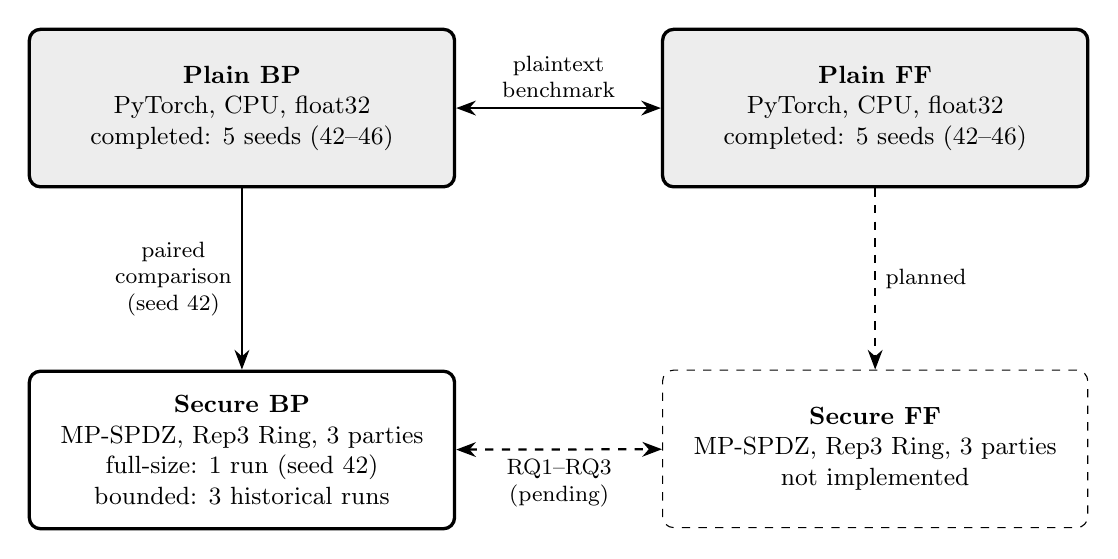
\begin{tikzpicture}[
  track/.style={draw, rounded corners, align=center, minimum width=5.4cm, minimum height=2.0cm, font=\small},
  done/.style={track, very thick, fill=black!7},
  partial/.style={track, very thick},
  todo/.style={track, dashed},
  link/.style={-{Stealth[length=2.5mm]}, thick},
  biglink/.style={{Stealth[length=2.5mm]}-{Stealth[length=2.5mm]}, thick},
  lab/.style={font=\footnotesize, align=center}
]
\node[done] (pbp) {\textbf{Plain BP}\\PyTorch, CPU, float32\\completed: 5 seeds (42--46)};
\node[done, right=2.6cm of pbp] (pff) {\textbf{Plain FF}\\PyTorch, CPU, float32\\completed: 5 seeds (42--46)};
\node[partial, below=2.3cm of pbp] (sbp) {\textbf{Secure BP}\\MP-SPDZ, Rep3 Ring, 3 parties\\full-size: 1 run (seed 42)\\bounded: 3 historical runs};
\node[todo, below=2.3cm of pff] (sff) {\textbf{Secure FF}\\MP-SPDZ, Rep3 Ring, 3 parties\\not implemented};
\draw[biglink] (pbp) -- node[lab, above]{plaintext\\benchmark} (pff);
\draw[link] (pbp) -- node[lab, left]{paired\\comparison\\(seed 42)} (sbp);
\draw[link, dashed] (pff) -- node[lab, right]{planned} (sff);
\draw[biglink, dashed] (sbp) -- node[lab, below]{RQ1--RQ3\\(pending)} (sff);
\end{tikzpicture}
\caption{The four experimental tracks and their status on 16 November 2026. Solid boxes: completed evidence; thick unfilled box: partial evidence; dashed: not yet implemented.}
\label{fig:method-tracks}
\end{figure}

\section{Learning Rule versus Secure-Computation Protocol}\label{sec:method-separation}
Two layers of the system are kept apart throughout the thesis. The \emph{learning rule} (\ac{bp} or \ac{ff}) defines which quantities are computed and how parameters are updated. The \emph{secure-computation protocol} (here, MP-SPDZ's three-party replicated-ring protocol) defines how each arithmetic or nonlinear operation is evaluated on secret-shared values, and therefore what each operation costs. A change at one layer is not a change at the other. In particular, rewriting secure \ac{bp} from scalar loops into matrix products (Chapter~\ref{chap:impl}) changes the cost of evaluating \ac{bp} under the same protocol, but the program still implements \ac{bp}: the same forward pass, the same softmax cross-entropy loss, the same backward recursion and the same \ac{sgd} update. Conversely, the research question about \ac{ff} concerns a change of learning rule under a fixed protocol. Any comparison of \ac{bp} and \ac{ff} under \ac{mpc} must therefore hold the protocol, threat model, arithmetic and implementation style (for example, matrix formulation) constant, or the effect of the learning rule cannot be separated from the effect of the implementation.

\section{Comparisons and Controlled Variables}\label{sec:method-comparisons}
The design calls for several distinct comparisons. They control different variables and support different claims, and they are kept separate in the results. Table~\ref{tab:method-comparisons} lists them with what is matched and what differs.

\begin{table}[ht]
\centering
\small
\begin{tabular}{@{}>{\raggedright\arraybackslash}p{2.6cm}>{\raggedright\arraybackslash}p{4.4cm}>{\raggedright\arraybackslash}p{4.3cm}>{\raggedright\arraybackslash}p{2.4cm}@{}}
\toprule
Comparison & Matched & Differs & Status \\
\midrule
C1: Plain BP vs Plain FF & Data split, seeds 42--46, hidden widths, batch size, number of epochs per trained unit, CPU software stack & Learning rule; parameters (118{,}282 vs 116{,}992); learning rate; optimizer updates (200 vs 400); presentations; inference procedure & Completed (5 seeds) \\
C2: Plain BP vs Secure BP (seed 42) & Split, sample order, initial parameters, architecture, loss, learning rate, batch schedule, epochs, evaluated checkpoint (epoch 5) & Arithmetic (float32 vs fixed point with probabilistic truncation); execution environment; nonlinear approximations & Completed (1 seed) \\
C3: Secure BP vs Secure FF & Planned: framework, protocol, threat model, arithmetic, data, host, implementation style & Learning rule and its budget & Not started \\
C4: Secure FF vs modified Secure FF & Planned: everything except the modification & Modification (with ablation) & Not started \\
Historical: A0, A1, BP-COMP-001 & 784--8--10 network, 90/30/30 subset, protocol & Ordering, initialisation, ReLU derivative, capture coverage & Completed; not compared causally \\
\bottomrule
\end{tabular}
\caption{Comparisons in the study, the variables each one controls, and their status.}
\label{tab:method-comparisons}
\end{table}

Comparison C2 deliberately crosses execution modes: it asks whether the secure implementation reproduces the plaintext learning trajectory for the same seed. It is a correctness and fidelity check, not a statement that secure training is equivalent to plaintext training in general. Hardware is not one of the controlled variables of C2: the plaintext benchmark records its software stack but not its processor, and the secure run records only that all parties ran on the local host (Section~\ref{sec:setup-env}). Runtime is therefore not compared across execution modes. For the planned comparison C3, the design calls for at least five seeds for utility and three repetitions for timing. The secure results available today are single runs and do not yet satisfy this requirement.

\section{Algorithm-Specific Training Budgets}\label{sec:method-budget}
\ac{bp} and \ac{ff} cannot be trained with identical procedures, so ``matched settings'' cannot mean identical work. In the plaintext benchmark, \ac{bp} trains the whole 784--128--128--10 network end to end for five epochs: 40 mini-batches per epoch (39 of 128 examples and one of 8) give $5\times40=200$ optimizer updates and $5\times5{,}000=25{,}000$ example presentations. \ac{ff} trains a 784--128--128 network greedily, one layer at a time: layer~1 is trained for five epochs, then frozen, and layer~2 is trained for five epochs on the normalised output of layer~1. Each mini-batch is presented once with the correct label (positive) and once with a uniformly random wrong label (negative), so \ac{ff} performs $2\times5\times40=400$ optimizer updates and $2\times2\times5\times5{,}000=100{,}000$ presentations, and every presentation of a training example to layer~2 also requires a forward pass through the frozen layer~1. \ac{ff} uses learning rate $0.01$, \ac{bp} uses $0.05$. At inference, \ac{bp} needs one forward pass per example, whereas \ac{ff} needs one pass per candidate label (ten passes) and chooses the label with the highest goodness accumulated over both layers. These differences are documented rather than equalised; differences in accuracy or time between the plaintext methods are therefore not attributed to the learning rule alone, and the budget of each method must be reported again with the secure comparison.

\section{Protocol, Threat Model and Fixed-Point Configuration}\label{sec:method-protocol}
All secure experiments use MP-SPDZ v0.4.4 \cite{keller2020mpspdz} at commit \texttt{113c4e47\allowbreak dd94bca9\allowbreak ecab029d\allowbreak 2f0abe64\allowbreak 9bea5c52}, with the three-party, semi-honest, honest-majority replicated-ring protocol (Rep3 Ring) over a 64-bit ring: at most one of the three parties may be corrupted, and a corrupted party is assumed to follow the protocol. Fixed-point numbers use \texttt{sfix(16,31)}: 16 fractional bits and 31 bits in total, giving a nominal range of about $[-16384,16384)$ and a quantisation step of $2^{-16}$ (Section~\ref{sec:bg-fixed}). For this protocol the MP-SPDZ compilation path enables probabilistic truncation and a three-way share split (\texttt{use\_trunc\_pr} and \texttt{use\_split(3)}); these are defaults of the execution path and not separately tuned choices. The compiler output lists 7{,}424{,}425 integer probabilistic truncations for the bounded runs A1 and BP-COMP-001 and 91{,}680{,}035 for the full-size run. The log of the historical run A0 instead ends with MP-SPDZ's suggestion to enable these two options, which indicates that A0 was executed without them. The deterministic alternative \texttt{sfix.round\_nearest} was not used, and no claim of zero leakage is made.

All secure runs since A1 also print the virtual-machine message that the computation domain is too small for low-round truncation and would need at least 103 bits. A reading of the pinned source (Section~\ref{sec:disc-trunc}) indicates that the message reports which truncation variant could not be used; its numerical and security implications for the executed variant have not been analysed and are listed as an open limitation. A separate malicious-security protocol (MASCOT) was explored in a tutorial during environment setup but is not the protocol of any reported experiment. Security statements apply only to this configuration.

\section{Historical Bounded Secure BP Study}\label{sec:method-scenario}
The first secure \ac{bp} experiments were deliberately small so that end-to-end secure runs were feasible with a scalar implementation. They are retained as development and validation milestones and are not combined with the full-size experiment.

\paragraph{Scenario.} A 784--8--10 fully connected network (6{,}370 trainable parameters, ReLU hidden layer, linear output layer) is trained on a 90/30/30 train/validation/test subset of MNIST. Three parties each own 30 training, 10 validation and 10 test examples; ownership is assigned by sample index modulo three, with three training examples per class and one validation and one test example per class for each party. Each mini-batch has size three, one example from each party, which gives 30 mini-batches per epoch; three epochs make 90 stochastic-gradient updates at learning rate $0.05$ without momentum or weight decay. Softmax cross-entropy is computed in a numerically stable form, and only aggregate results (losses and correct counts) are released.

\paragraph{Ordering of training examples.} An audit of the historical runs A0 and A1 found that their batches were class-major: each batch contained three examples of the same class, and the same fixed schedule was repeated in every epoch, with no example skipped or duplicated. Long runs of one class can bias \ac{sgd}; the effect on the historical runs has not been isolated. For the comparison-readiness run BP-COMP-001, a deterministic per-party shuffle of the training order in every epoch was introduced. It preserves the selected sample indices, the party ownership, the 90/30/30 split and the one-example-per-party-per-batch structure, and it is reproducible from an ordering seed (42042).

\paragraph{Parameter initialisation.} The historical runs used a public, deterministic initialisation of the weights provided by one party, $W_{ij}=(i-j)/1000$, with zero biases; this is neither private nor random. Candidate schemes were compared in controlled plaintext diagnostics C0--C3, and configuration C3 was selected for BP-COMP-001. C3 combines per-party shuffled ordering, He initialisation of the hidden layer \cite{he2015delving}, Xavier (Glorot) uniform initialisation of the output layer \cite{glorot2010understanding} and zero biases, with initialisation seed 42: the 784$\times$8 hidden weights are drawn from a normal distribution with variance $2/784$ and the $8\times10$ output weights uniformly from $[-\ell,\ell]$ with $\ell=\sqrt{6/(8+10)}$. The detailed C0--C2 results are not part of the archived artifacts, so no statement is made that C3 outperformed every alternative. \emph{Ordering and initialisation were changed together in C3}, so any difference between the historical runs and BP-COMP-001 cannot be attributed to either factor alone.

\section{Full-Size Matched Secure BP Experiment}\label{sec:method-full}
The full-size experiment (identifier SECURE-BP-MATCHED-v1, batched-matrix program) is designed to reproduce the Plain BP baseline configuration under \ac{mpc} as closely as the arithmetic allows, so that comparison C2 is a paired comparison for one seed.

\paragraph{Data and split.} MNIST is split with the same function as the plaintext baseline: 5{,}000 training and 1{,}000 validation examples from a seeded permutation of the official training set, and 1{,}000 test examples from positions 1{,}000--1{,}999 of a seeded permutation of the official test set (positions 0--999 are excluded because they had been exposed in early development).

\paragraph{Order, batches and initialisation.} The training order is the order produced by the plaintext baseline's seeded PyTorch data loader (batch size 128, shuffling, seed 42), with the loader state continuing across the five epochs. Each epoch has 39 batches of 128 examples and one final batch of 8, so five epochs give 200 updates. The initial parameters are the PyTorch default initialisation of the same model after setting seed 42, transposed from PyTorch's output-by-input layout to the input-by-output layout of the secure program. The input bundle records SHA-256 hashes of the five epoch orders, and an independent verifier checked that the bundle reproduces the baseline order, ownership and parameter layout (Section~\ref{sec:impl-provenance}).

\paragraph{Parties and disclosure.} Party~0 inputs the initial parameters. Every training, validation and test example is input by the party whose index equals the example's position modulo three, so each party owns about one third of the data. Features, labels, activations, gradients and parameters remain secret-shared throughout training; only the mean training loss of each epoch and the aggregate validation and test loss and correct counts are opened. The initial parameters are derived from a public seed and are therefore not private to party~0; the experiment protects the training data, not the initialisation.

\paragraph{Learning rule.} Training is plain \ac{bp} with mini-batch \ac{sgd} at learning rate $0.05$, no momentum and no weight decay; the gradient of each batch is averaged over the actual batch size, so the final batch is divided by 8, as in PyTorch.

\section{Evaluation Policy}\label{sec:method-eval}
The plaintext benchmark selects, for every seed, the checkpoint with the highest validation accuracy over the training epochs and reports its test accuracy. The secure program evaluates only the final (epoch-5) model. For seed 42, the plaintext baseline selected epoch 5, so comparison C2 compares the same checkpoint. For the five-seed plaintext aggregate this is not the case: seed 44 of Plain BP selected epoch 3, and every Plain FF seed selected the first epoch of layer~2. Five-seed plaintext aggregates are therefore not directly comparable with a future multi-seed secure aggregate unless the same checkpoint policy is used; this choice must be fixed before further secure seeds are run.

\section{Verification and Measurement Definitions}\label{sec:method-measure}
Correctness of the secure programs is checked at several levels: by an aggregate verifier for the bounded runs; by a strict ReLU-boundary program on public values; by matched plaintext FP64 references (for BP-COMP-001, for a single batch of the matrix prototype, and for the one-epoch smoke run of the full-size program); and, for the full-size run, by the paired comparison C2 with the recorded Plain BP run. These comparisons test close agreement of aggregate or intermediate quantities; they do not establish bit-exact equivalence or identical predictions.

Cost is measured with the following definitions, applied per experiment:
\begin{itemize}
  \item \emph{MP-SPDZ time}: the \texttt{Time} value printed by party~0. The run output states that it includes preprocessing (offline phase). It is started after the program has been loaded and does not include compilation.
  \item \emph{External elapsed time}: the wall-clock time measured by \texttt{/usr/bin/time -v} around the command that compiles the program and launches the three parties; available for the full-size and smoke runs only.
  \item \emph{Party-0 data sent} and \emph{party-0 rounds}: the volume sent by party~0 and its approximate count of communication rounds, as printed by the run.
  \item \emph{Global data sent}: the sum of the data sent by all three parties, as printed by the run.
  \item \emph{Compiler VM rounds}: the virtual-machine round count printed by the compiler; a compile-time statistic.
  \item \emph{Maximum resident set size}: as printed by \texttt{/usr/bin/time -v} for the timed process tree.
\end{itemize}
Runs whose measurement boundaries or capture coverage differ are not compared.

\section{Planned Secure FF Methodology}\label{sec:method-planned}
The design continues with a secure \ac{ff} implementation on the same data split, protocol, threat model, fixed-point type, host and matrix implementation style as the full-size secure \ac{bp} program, starting from the Plain FF configuration (784--128--128, label embedded in the first ten input pixels, L2 normalisation between layers, goodness as the sum of squared ReLU activities, threshold $2.0$, softplus local loss, per-layer \ac{sgd}, uniformly random wrong labels, inference over all candidate labels). Design questions that must be settled before implementation include how the wrong label of a negative example is generated without revealing the true label, how the softplus loss and the L2 normalisation are evaluated (exactly or by approximation), how inference over ten candidate labels is batched, and which checkpoint is evaluated. After a matched comparison with repeated runs (C3), both secure methods will be profiled per operation, and one bottleneck-motivated \ac{mpc}-aware modification of \ac{ff} will be evaluated against the unmodified baseline with an ablation (C4). None of these steps has been carried out at the time of writing, and no result of them is reported in this thesis.

\chapter{System Design and Implementation}\label{chap:impl}
\sloppy

This chapter describes the implementations behind the four experimental tracks as they exist on 16 November 2026: the plaintext baselines, the historical bounded secure \ac{bp} programs, and the batched-matrix secure \ac{bp} program used for the full-size run. Secure \ac{ff} has not been implemented. All code, configurations and recorded results are kept in the project repository; paths below are relative to its root.

\section{Software Environment}\label{sec:impl-env}
The secure computation uses MP-SPDZ v0.4.4 at the commit given in Section~\ref{sec:method-protocol}, built locally with the replicated-ring party binary (\texttt{replicated-ring-party.x}). The plaintext baselines are implemented in Python with PyTorch on CPU (Python 3.14.4, PyTorch 2.14.1+cpu, four threads, as recorded in the benchmark metadata). Data preparation, input generation and verification scripts are written in Python. The execution environment of the secure runs is described in Section~\ref{sec:setup-env}.

\section{Plaintext Baselines}\label{sec:impl-plain}
\paragraph{Plain BP} (\texttt{src/\allowbreak baselines/\allowbreak bp.py}) is a PyTorch \texttt{Sequential} model 784--128--128--10 with ReLU hidden layers and a linear output layer (118{,}282 parameters), initialised with the PyTorch default after \texttt{torch.manual\_seed(seed)}. It is trained with cross-entropy loss and \ac{sgd} at learning rate $0.05$ (no momentum) with batch size 128 for five epochs; the training loader shuffles with a generator seeded by the run seed. After every epoch the validation accuracy is computed and the best checkpoint is kept.

\paragraph{Plain FF} (\texttt{src/\allowbreak baselines/\allowbreak ff.py}) uses two fully connected layers 784--128--128 (116{,}992 parameters) with PyTorch default initialisation. The label is embedded by overwriting the first ten input pixels with a one-hot code. Each layer computes $\mathbf{h}=\mathrm{ReLU}(W\mathbf{x}+\mathbf{b})$, its goodness is $g=\sum_j h_j^2$ (computed before normalisation), and its output is L2-normalised before it is passed on. The local loss is $\mathrm{softplus}(\theta-g_{+})+\mathrm{softplus}(g_{-}-\theta)$, averaged over the batch, with threshold $\theta=2.0$ (Equations~\eqref{eq:ff-loss-pos}--\eqref{eq:ff-loss-neg}). Negative examples use a uniformly random wrong label drawn from a separately seeded generator. Layers are trained greedily, five epochs each, with one \ac{sgd} optimizer per layer at learning rate $0.01$ and batch size 128. Inference evaluates all ten candidate labels and selects the label with the highest goodness summed over both layers. During training of layer~2, the validation accuracy after every epoch selects the reported checkpoint.

\paragraph{Benchmark harness.} \texttt{scripts/\allowbreak benchmark.py} runs both methods on the same split for seeds 42--46 with three timing repetitions per seed and writes \texttt{results/\allowbreak benchmarks/\allowbreak plaintext/} (\texttt{runs.csv}, \texttt{summary.csv}, \texttt{metadata.json}). The metadata records SHA-256 hashes of the two baseline sources and the harness.

\section{Historical Bounded Secure BP Programs}\label{sec:impl-secure}
The first secure program is written in the MP-SPDZ high-level language with scalar loops. A data-preparation script (\texttt{prepare\_\allowbreak mpc\_\allowbreak data.py}) selects the bounded MNIST subset, assigns ownership and writes the per-party input files together with metadata and file hashes. The training program (\texttt{bp\_\allowbreak train.mpc}) performs the forward pass, softmax cross-entropy, the backward pass with the strict ReLU derivative ($0<z$) and \ac{sgd} updates for the 784--8--10 network; a run script invokes compilation and execution for the replicated-ring protocol and logs the output. The comparison-readiness pass added a run configuration (\texttt{bp\_\allowbreak comparison.yaml}), a plaintext FP64 reference implementation (\texttt{bp\_\allowbreak training\_\allowbreak reference.py}) with tests, a strict ReLU edge-case program (\texttt{relu\_\allowbreak strict\_\allowbreak edge.mpc}) with its verifier and a report. The raw artifacts of BP-COMP-001 (input files, initial parameters, metadata, FP64 reference, runtime log) are stored under \texttt{results/\allowbreak mpc/\allowbreak bp/\allowbreak comparison\_\allowbreak baseline/\allowbreak BP-COMP-001/}. Historical artifacts of the earlier runs were left unchanged; a mismatch between the runtime-log checksum embedded in the metadata of A0 and the actual checksum of its log is documented, and the raw files are preserved unaltered.

\section{From Scalar Loops to Matrix Products}\label{sec:impl-scalar}
To scale secure \ac{bp} to the plaintext configuration, the scalar implementation was first generalised: a shared template (\texttt{bp\_\allowbreak secure\_\allowbreak template.mpc.in}) renders both the bounded profile and a full-size scalar profile (\texttt{bp\_\allowbreak matched.mpc}) for 784--128--128--10 with the 39$\times$128 + 8 batch schedule. This program is a correct reference implementation, but it is not executable in practice. Compile-only statistics from the pinned compiler (Table~\ref{tab:impl-scalar-matrix}) show about $2.0\times10^{10}$ virtual-machine rounds and $6.6\times10^{9}$ probabilistic truncations, because every scalar product is truncated and scheduled separately. A nine-sample diagnostic of the scalar program did not finish within a 600-second limit.

The batched-matrix program (\texttt{mpc/\allowbreak programs/\allowbreak bp/\allowbreak bp\_\allowbreak matched\_\allowbreak matrix.mpc}) implements the same experiment with MP-SPDZ's native matrix products. For the same network, data and schedule, its compiler output lists 5{,}638{,}872 virtual-machine rounds and 91{,}680{,}035 probabilistic truncations, about $3{,}500\times$ fewer rounds and $72\times$ fewer truncations. These are compile-time upper-bound statistics, not measured costs; they explain why the matrix program was used for the full run.

\begin{table}[ht]
\centering
\small
\begin{tabular}{@{}>{\raggedright\arraybackslash}p{6.0cm}rr@{}}
\toprule
Compiler statistic (\texttt{-E ring -l -M}) & Scalar (\texttt{bp\_matched}) & Matrix (\texttt{bp\_matched\_matrix}) \\
\midrule
Virtual-machine rounds & 19{,}965{,}875{,}172 & 5{,}638{,}872 \\
Integer probabilistic truncations & 6{,}638{,}164{,}835 & 91{,}680{,}035 \\
Bit triples & 1{,}761{,}310{,}000 & 933{,}945{,}000 \\
Integer simple multiplications & 6{,}631{,}571{,}400 & 23{,}454{,}000 \\
Integer dot products & 0 & 37{,}185{,}200 \\
Matrix multiplications (all shapes) & 0 & 1{,}660 \\
\bottomrule
\end{tabular}
\caption{Compile-only statistics of the scalar and batched-matrix full-size secure \ac{bp} programs (pinned MP-SPDZ compiler; records in \texttt{results/mpc/bp/matrix\_matched\_v1\_preflight/}). Statistics are the compiler's ``requires at most'' counts, not run-time measurements.}
\label{tab:impl-scalar-matrix}
\end{table}

\section{Batched-Matrix Secure BP Program}\label{sec:impl-matrix}
\paragraph{Parameters and layout.} The weights are declared as secret fixed-point matrices $W^{(1)}\in\mathbb{R}^{784\times128}$, $W^{(2)}\in\mathbb{R}^{128\times128}$ and $W^{(3)}\in\mathbb{R}^{128\times10}$ in input-by-output, row-major layout, with bias vectors $\mathbf{b}^{(l)}$. PyTorch stores the weight of a linear layer as output-by-input, so the input generator transposes each weight matrix; biases are unchanged. With batch rows as matrix rows, a layer is $Z=XW+\mathbf{1}\mathbf{b}^\top$, which is the row-wise form of Equation~\eqref{eq:mlp-pre}.

\paragraph{Batch processing.} Three sets of buffers have compile-time row counts: 128 for full training batches, 8 for the final batch and 100 for evaluation chunks. Loading a batch reads, in a sequential loop, the 784 pixel values and the 10-element one-hot label of each example from the input stream of its owner, so that the per-party streams are consumed in exactly the order in which they were written. Each epoch runs 39 full batches in a run-time loop followed by the final batch of eight with its own buffers.

\paragraph{Forward pass and loss.} Each layer computes a native matrix product (\texttt{direct\_mul}) followed by a row-wise bias addition. The ReLU layer computes the mask $M=[Z>0]$ by secure comparison, stores it, and sets $H=Z\odot M$; the stored mask is reused as the derivative in the backward pass, so $\sigma'(0)=0$ as in the strict convention of Section~\ref{sec:bg-bp}. The loss is computed per row in numerically stable form, $\mathcal{L}=\log\sum_k e^{z_k-s}+s-z_y$ with a shift $s$ supplied by MP-SPDZ's softmax helper, using the library's secure exponentiation, logarithm and division; the softmax probabilities $P$ are stored for the backward pass.

\paragraph{Backward pass and update.} The output error is $D^{(3)}=P-Y$. Hidden errors use products with the transposed weights (\texttt{direct\_mul\_trans}), $D^{(2)}=(D^{(3)}W^{(3)\top})\odot M^{(2)}$ and $D^{(1)}=(D^{(2)}W^{(2)\top})\odot M^{(1)}$. Weight gradients are products of transposed activations with errors, $\nabla W^{(l)}=A^{(l-1)\top}D^{(l)}$ (\texttt{direct\_trans\_mul}), accumulated without intermediate truncation and reduced once per output element; bias gradients are column sums of $D^{(l)}$. Each parameter is then updated as $\theta\leftarrow\theta-(\eta\nabla\theta)\cdot(1/B)$ with $\eta=0.05$ and $B$ the actual batch size (128 or 8). The factor $1/B$ is a public constant that is exactly representable for both batch sizes; a project analysis found that the single constant $0.05/128$ would be rounded to 26 quanta of $2^{-16}$ instead of 25.6, a learning-rate bias of about 1.6\%, which this form avoids. Parameters persist across batches and epochs. Algorithm~\ref{alg:impl-batch} summarises one training batch.

\begin{algorithm}[ht]
\caption{One training batch of the batched-matrix secure \ac{bp} program (all values secret-shared).}
\label{alg:impl-batch}
\begin{algorithmic}[1]
\STATE Load $B$ examples into $X\in\mathbb{R}^{B\times784}$, $Y\in\{0,1\}^{B\times10}$; example $r$ is input by party $(\mathit{start}+r) \bmod 3$
\STATE $Z^{(1)} \leftarrow XW^{(1)}+\mathbf{1}\mathbf{b}^{(1)\top}$; \quad $M^{(1)}\leftarrow[Z^{(1)}>0]$; \quad $H^{(1)}\leftarrow Z^{(1)}\odot M^{(1)}$
\STATE $Z^{(2)} \leftarrow H^{(1)}W^{(2)}+\mathbf{1}\mathbf{b}^{(2)\top}$; \quad $M^{(2)}\leftarrow[Z^{(2)}>0]$; \quad $H^{(2)}\leftarrow Z^{(2)}\odot M^{(2)}$
\STATE $Z^{(3)} \leftarrow H^{(2)}W^{(3)}+\mathbf{1}\mathbf{b}^{(3)\top}$
\STATE For each row: stable softmax $P$ and cross-entropy; add the row loss to the epoch total
\STATE $D^{(3)}\leftarrow P-Y$; \quad $D^{(2)}\leftarrow (D^{(3)}W^{(3)\top})\odot M^{(2)}$; \quad $D^{(1)}\leftarrow (D^{(2)}W^{(2)\top})\odot M^{(1)}$
\STATE $\nabla W^{(3)}\leftarrow H^{(2)\top}D^{(3)}$; \quad $\nabla W^{(2)}\leftarrow H^{(1)\top}D^{(2)}$; \quad $\nabla W^{(1)}\leftarrow X^{\top}D^{(1)}$ (one truncation per element)
\STATE $\nabla\mathbf{b}^{(l)}\leftarrow$ column sums of $D^{(l)}$
\STATE $\theta \leftarrow \theta - (0.05\,\nabla\theta)\cdot(1/B)$ for every weight matrix and bias vector
\end{algorithmic}
\end{algorithm}

\paragraph{Evaluation and disclosure.} After five epochs, the final model is evaluated on the 1{,}000 validation and 1{,}000 test examples in chunks of 100 rows. The prediction is the argmax of the logits, as in the plaintext baseline, and is compared with the argmax of the one-hot label inside \ac{mpc}. Only the mean training loss of each epoch and the mean loss and number of correct predictions on the validation and test sets are revealed.

\paragraph{Differences from the scalar program.} The matrix program differs from the scalar program only in numerical detail: dot products are truncated once per output element instead of once per product, the update uses the exact $1/B$ factor, the ReLU mask is computed once and reused, and evaluation uses the argmax of the logits. None of these changes the learning rule; both programs implement mini-batch \ac{bp} with \ac{sgd}, and each is compared with an FP64 reference rather than with the other.

\section{Input Generation, Ownership and Provenance}\label{sec:impl-provenance}
The three per-party input files for the full-size run are produced by \texttt{scripts/\allowbreak prepare\_\allowbreak secure\_\allowbreak bp\_\allowbreak matched.py}, which reuses the baseline split function and data loader to write each party's stream in consumption order: party~0 first writes all 118{,}282 initial parameters, and then every party writes, for each epoch and each training position it owns, 784 pixel values and 10 label values, followed by its validation and test examples (Figure~\ref{fig:impl-parties}). The resulting bundle (\texttt{SECURE-BP-MATCHED-v1\_seed42\_corrected}) contains 7{,}266{,}664, 7{,}146{,}794 and 7{,}142{,}824 input values for parties 0, 1 and 2, together with \texttt{metadata.json}, \texttt{parameters.json} and \texttt{verification\_summary.json}. The bundle name records that two errors of an earlier generator were corrected before any full run: the training order initially did not reproduce the plaintext data loader's internal use of its random generator, and the weight matrices were initially not transposed.

The independent verifier \texttt{scripts/\allowbreak verify/\allowbreak verify\_\allowbreak secure\_\allowbreak bp\_\allowbreak inputs.py} parses every stream and reports \texttt{all\_pass: true} for all its checks: all tokens consumed with the expected per-party counts, the five epoch orders equal to the baseline order and ownership, validation and test order and ownership, transposed initial-parameter layout, and input hashes matching the metadata. The program and input hashes recorded for the run are listed in Appendix~\ref{app:manifest}. The bundle metadata records that it was generated from repository commit \texttt{974e202} with uncommitted changes in the working tree; the matrix program, the verifier and the evidence record were committed afterwards (commit \texttt{ef00de1}), and the committed program file has the SHA-256 recorded for the run.

\begin{figure}[ht]
\centering
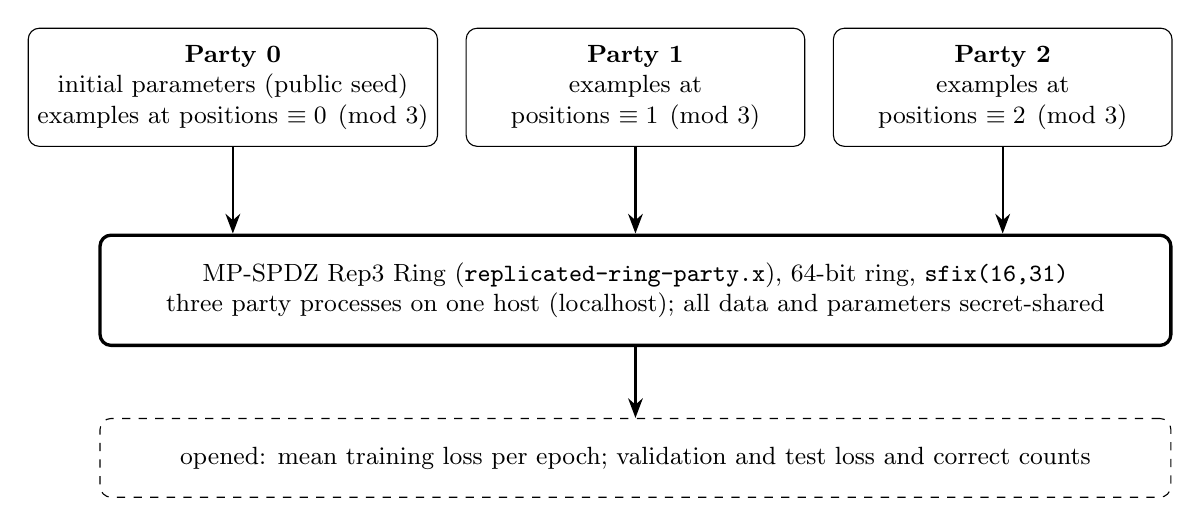
\begin{tikzpicture}[
  party/.style={draw, rounded corners, align=center, minimum width=4.3cm, minimum height=1.5cm, font=\small},
  core/.style={draw, very thick, rounded corners, align=center, minimum width=13.6cm, minimum height=1.4cm, font=\small},
  outbox/.style={draw, dashed, rounded corners, align=center, minimum width=13.6cm, minimum height=1.0cm, font=\small},
  link/.style={-{Stealth[length=2.5mm]}, thick}
]
\node[party] (p0) {\textbf{Party 0}\\initial parameters (public seed)\\examples at positions $\equiv0 \pmod 3$};
\node[party, right=0.35cm of p0] (p1) {\textbf{Party 1}\\examples at\\positions $\equiv1 \pmod 3$};
\node[party, right=0.35cm of p1] (p2) {\textbf{Party 2}\\examples at\\positions $\equiv2 \pmod 3$};
\node[core, below=1.1cm of p1] (mpc) {MP-SPDZ Rep3 Ring (\texttt{replicated-ring-party.x}), 64-bit ring, \texttt{sfix(16,31)}\\three party processes on one host (localhost); all data and parameters secret-shared};
\node[outbox, below=0.9cm of mpc] (res) {opened: mean training loss per epoch; validation and test loss and correct counts};
\draw[link] (p0) -- (p0 |- mpc.north);
\draw[link] (p1) -- (mpc);
\draw[link] (p2) -- (p2 |- mpc.north);
\draw[link] (mpc) -- (res);
\end{tikzpicture}
\caption{Inputs, protocol and disclosure of the full-size secure \ac{bp} run. Ownership by position modulo three simulates three data owners; all three processes ran on the same host.}
\label{fig:impl-parties}
\end{figure}

\section{Verification Before the Full Run}\label{sec:impl-verify}
The full-size program was introduced through a sequence of checks of increasing scope. These are implementation-verification evidence, not training results.
\begin{enumerate}
  \item \emph{Offline references.} A float64 Python simulator that consumes the party streams exactly as the program does reproduces PyTorch float64 \ac{sgd} on the baseline data loader (parameter differences of at most $1.1\times10^{-16}$ after every epoch) and the recorded float32 Plain BP losses to the displayed digits. A fixed-point emulation with 16 fractional bits and probabilistic rounding (but floating-point exp, log and division) predicted an epoch-5 training loss within about $10^{-4}$ of float64, 766--767 correct validation examples and 772 correct test examples. The repository's unit tests (68 at the time of the pre-run report) were reported as passing; they were not re-run for this thesis version.
  \item \emph{Single-batch MPC audit.} A diagnostic variant of a batch-size-3 matrix prototype on the full architecture revealed all intermediate tensors of one training step. Against an FP64 reference, all 24 audited tensors matched in shape and orientation, the predictions matched, and the largest absolute error over 238{,}964 values was $2.2\times10^{-4}$.
  \item \emph{One-epoch smoke run.} A smoke profile of the full program (one epoch over 264 training examples in batches of 128, 128 and 8; 100 validation and 100 test examples) ran under MPC on 15 November 2026. It printed a training loss of 2.30479, a validation loss of 2.29572 with 15/100 correct and a test loss of 2.28882 with 19/100 correct, against FP64 reference values of 2.30485, 2.29580 (15/100) and 2.28888 (19/100), all within the pre-registered tolerance of $8.6\times10^{-5}$ and with exactly the expected counts.
\end{enumerate}

\section{MP-SPDZ Integration and Run Hygiene}\label{sec:impl-integration}
The secure programs are compiled and executed with MP-SPDZ's \texttt{compile-run.py} using the options \texttt{-l -M -E ring}, which select the ring-protocol optimisations and start the three replicated-ring parties on the local host. For the matrix runs, the input bundle is passed to the parties with the runtime option \texttt{-IF} (input-file prefix), so that the existing files in MP-SPDZ's \texttt{Player-Data} directory are not overwritten. Before the full run, \texttt{Player-Data} was copied to a separate backup directory (33 files, 40{,}492{,}581 bytes); this directory contains key material and preprocessing state and is not part of the thesis evidence package. The run output was written to a new, dedicated run directory.

\section{Current Implementation Status}\label{sec:impl-status}
Plaintext \ac{bp} and \ac{ff} baselines exist and have been benchmarked. Secure \ac{bp} exists as historical bounded scalar programs, a full-size scalar reference program that is not executable in practice, and a batched-matrix program that has completed one full-size run. A secure \ac{ff} implementation has not been started, per-operation profiling of either method has not been done, and no \ac{mpc}-aware \ac{ff} modification has been implemented. The core secure \ac{bp}-versus-\ac{ff} comparison has therefore not been carried out.

\chapter{Experimental Setup}\label{chap:setup}

This chapter lists the configurations of all experiments reported in Chapter~\ref{chap:results}. The plaintext benchmark, the historical bounded secure runs and the two full-size secure runs (Secure BP and Secure FF) are separate experimental regimes and are described in separate tables. Measurement definitions are given in Section~\ref{sec:method-measure}.

\section{Data}\label{sec:setup-data}
All experiments use MNIST (28$\times$28 grey-scale digits, 784 input values, 10 classes). Table~\ref{tab:setup-data} lists the splits.

\begin{table}[ht]
\centering
\small
\begin{tabular}{@{}>{\raggedright\arraybackslash}p{3.6cm}>{\raggedright\arraybackslash}p{4.4cm}>{\raggedright\arraybackslash}p{5.8cm}@{}}
\toprule
Regime & Train / validation / test & Source of the examples \\
\midrule
Plaintext benchmark (Plain BP, Plain FF) & 5{,}000 / 1{,}000 / 1{,}000 & Train and validation: first 5{,}000 and next 1{,}000 positions of a seed-42 permutation of the official training set; test: positions 1{,}000--1{,}999 of a seed-42 permutation of the official test set \\
Full-size Secure BP & 5{,}000 / 1{,}000 / 1{,}000 & Same split function and indices as the plaintext benchmark \\
Full-size Secure FF & 5{,}000 / 1{,}000 / 1{,}000 & Same split function and indices as the plaintext benchmark (checked by an independent verifier against the dataset and the Secure BP bundle); seed 42 \\
Bounded Secure BP (A0, A1, BP-COMP-001) & 90 / 30 / 30 & Class-balanced subset, selection seed 42; 30 / 10 / 10 per party \\
\bottomrule
\end{tabular}
\caption{Data splits of the three experimental regimes.}
\label{tab:setup-data}
\end{table}

\section{Plaintext Benchmark}\label{sec:setup-plain}
Table~\ref{tab:setup-plain} gives the configuration of the plaintext benchmark (identifier PT-BENCH-v1, profile \texttt{project\_baseline\_standardized}).

\begin{table}[ht]
\centering
\small
\begin{tabular}{@{}>{\raggedright\arraybackslash}p{3.6cm}>{\raggedright\arraybackslash}p{5.0cm}>{\raggedright\arraybackslash}p{5.2cm}@{}}
\toprule
Item & Plain BP & Plain FF \\
\midrule
Architecture & 784--128--128--10, ReLU, linear output & 784--128--128, ReLU, L2 normalisation between layers \\
Parameters & 118{,}282 & 116{,}992 \\
Initialisation & PyTorch default, \texttt{manual\_seed(seed)} & PyTorch default, \texttt{manual\_seed(seed)} \\
Objective & Softmax cross-entropy & Per-layer softplus goodness loss, threshold 2.0 \\
Label handling & Target class & One-hot label in first 10 pixels; negatives with a uniformly random wrong label \\
Optimizer & \ac{sgd}, learning rate 0.05 & Per-layer \ac{sgd}, learning rate 0.01 \\
Batch size; epochs & 128; 5 & 128; 5 per layer, layers trained in sequence \\
Optimizer updates & 200 & 400 \\
Example presentations & 25{,}000 & 100{,}000 (positive and negative) \\
Inference & One forward pass, argmax of logits & Ten candidate-label passes, highest goodness summed over both layers \\
Checkpoint & Best validation accuracy over epochs & Best validation accuracy over layer-2 epochs \\
Seeds; repetitions & 42--46; 3 timing repetitions per seed & 42--46; 3 timing repetitions per seed \\
\bottomrule
\end{tabular}
\caption{Configuration of the plaintext benchmark PT-BENCH-v1.}
\label{tab:setup-plain}
\end{table}

\section{Historical Bounded Secure BP Runs}\label{sec:setup-bounded}
Table~\ref{tab:setup-secure} lists the configuration of the bounded secure \ac{bp} runs.

\begin{table}[ht]
\centering
\small
\begin{tabular}{@{}>{\raggedright\arraybackslash}p{4.3cm}>{\raggedright\arraybackslash}p{9.6cm}@{}}
\toprule
Item & Setting \\
\midrule
Framework, protocol & MP-SPDZ v0.4.4; Rep3 Ring; 3 parties; semi-honest, honest majority \\
Arithmetic & 64-bit ring; \texttt{sfix(16,31)}; probabilistic truncation and \texttt{use\_split(3)} for A1 and BP-COMP-001 (the A0 log suggests that these options were not enabled for A0) \\
Program & Scalar loops (\texttt{bp\_train.mpc}) \\
Model & 784--8--10 \ac{mlp}, ReLU hidden layer, linear output layer, 6{,}370 parameters \\
Data & MNIST subset: 90 train / 30 validation / 30 test; 30/10/10 per party \\
Training & Batch size 3 (one per party); 30 batches per epoch; 3 epochs; 90 updates; learning rate 0.05; no momentum or weight decay \\
Loss, output & Stable softmax cross-entropy; aggregate-only outputs \\
Historical runs (A0, A1) & Class-major batches; deterministic initialisation $(i-j)/1000$, zero biases \\
BP-COMP-001 & Per-party shuffled order (ordering seed 42042); He (hidden) and Xavier uniform (output) initialisation (seed 42); zero biases \\
Metrics & Validation/test correct out of 30; losses; MP-SPDZ time; global communication; compiler VM rounds \\
Repetitions & One run per configuration \\
Execution host & All three parties on one host (localhost) \\
\bottomrule
\end{tabular}
\caption{Configuration of the bounded secure \ac{bp} experiments.}
\label{tab:setup-secure}
\end{table}

\section{Full-Size Secure BP Run}\label{sec:setup-full}
Table~\ref{tab:setup-full} lists the configuration of the full-size run. All items were checked against the program source, the configuration file \texttt{configs/\allowbreak bp\_\allowbreak matched.yaml}, the input-bundle metadata and the run log.

\begin{table}[ht]
\centering
\small
\begin{tabular}{@{}>{\raggedright\arraybackslash}p{4.3cm}>{\raggedright\arraybackslash}p{9.6cm}@{}}
\toprule
Item & Setting \\
\midrule
Experiment & SECURE-BP-MATCHED-v1, batched-matrix program, seed 42 \\
Program & \texttt{mpc/programs/bp/bp\_matched\_matrix.mpc} \\
Framework, protocol & MP-SPDZ v0.4.4 (commit \texttt{113c4e47}); Rep3 Ring; 3 parties; semi-honest, honest majority \\
Arithmetic & 64-bit ring; \texttt{sfix(16,31)}; probabilistic truncation; \texttt{use\_split(3)} \\
Compile and run command & \texttt{compile-run.py -l -M -E ring bp\_matched\_matrix -- -IF \textless{}bundle\textgreater{}/Input} \\
Model & 784--128--128--10, ReLU hidden layers, linear output layer, 118{,}282 parameters \\
Initialisation & PyTorch default after seed 42, transposed to input-by-output layout; input by party 0 \\
Data & 5{,}000 / 1{,}000 / 1{,}000 (Table~\ref{tab:setup-data}); example owner = position modulo 3 \\
Order & Baseline seed-42 data loader order, state continued across epochs \\
Training & Batch size 128; 39 batches of 128 and one of 8 per epoch (40 batches); 5 epochs; 200 updates; \ac{sgd}, learning rate 0.05, no momentum or weight decay; gradients averaged over the actual batch size \\
Loss & Stable softmax cross-entropy \\
Evaluation & Final (epoch-5) model; argmax of logits; chunks of 100 \\
Disclosure & Mean training loss per epoch; validation and test mean loss and correct count \\
Repetitions & One run (seed 42); no timing repetitions \\
Date & 15 November 2026 (run directory timestamp 23:49:46 local time) \\
\bottomrule
\end{tabular}
\caption{Configuration of the full-size secure \ac{bp} run.}
\label{tab:setup-full}
\end{table}

\section{Full-Size Secure FF Run}\label{sec:setup-sff}
Table~\ref{tab:setup-sff} lists the configuration of the full-size Secure \ac{ff} run. The items were taken from the configuration file \texttt{configs/\allowbreak ff\_\allowbreak secure\_\allowbreak matched.yaml}, the program header and source, the command record and the run output. Where the Secure \ac{bp} and Secure \ac{ff} settings differ, the difference is intended (learning rule) or is a documented confound (Section~\ref{sec:method-sff}).

\begin{table}[htbp]
\centering
\small
\begin{tabular}{@{}>{\raggedright\arraybackslash}p{4.3cm}>{\raggedright\arraybackslash}p{9.6cm}@{}}
\toprule
Item & Setting \\
\midrule
Experiment & SECURE-FF-MATCHED-v1, profile \texttt{full}, seed 42; run directory \texttt{seed42\_run\_20261122\_212319} \\
Program & \texttt{mpc/programs/ff/ff\_matched.mpc} \\
Framework, protocol & MP-SPDZ v0.4.4 (commit \texttt{113c4e47}); Rep3 Ring; 3 parties; semi-honest, honest majority \\
Arithmetic & 64-bit ring; \texttt{sfix(16,31)}; default probabilistic truncation \\
Compile command & \texttt{compile.py -M -E ring ff\_matched} (no \texttt{-l}) \\
Run command & \texttt{Scripts/ring.sh ff\_matched -IF \textless{}bundle\textgreater{}/Input}, three party processes on \texttt{localhost} \\
Model & 784--128--128, ReLU, 116{,}992 parameters; no output layer \\
Initialisation & Plain FF model after \texttt{random.seed} and \texttt{torch.manual\_seed} with seed 42, transposed to input-by-output layout; input by party 0 \\
Data & 5{,}000 / 1{,}000 / 1{,}000 (Table~\ref{tab:setup-data}); record owner = position modulo 3 \\
Order & One seeded data loader iterated ten times; state continued across layers \\
Local objective & $\frac1B\sum\mathrm{softplus}(\theta-g^{+})+\frac1B\sum\mathrm{softplus}(g^{-}-\theta)$; $\theta=2.0$; goodness = sum of squared ReLU activations before normalisation \\
Normalisation & Stable max-scaled L2 normalisation between the layers \\
Negative labels & Uniformly random incorrect label, generated in \ac{mpc} (ten rejection-sampling tries of eight secret bits) \\
Optimizer & Per-layer \ac{sgd}, learning rate 0.01, no momentum or weight decay; update $\eta/B$ applied as $a\cdot2^{-s}$ \\
Batches & Batch size 128; 39 batches of 128 and one of 8 per epoch (40 batches); every example of a batch is presented once with its correct label (positive) and once with an incorrect label (negative), in one stacked matrix \\
Epochs and updates & 5 epochs for layer 1, then 5 epochs for layer 2 (layer 1 frozen); 200 updates per layer, 400 in total \\
Inference & Ten candidate labels, chunks of 50 samples, score = goodness of layer 1 + goodness of layer 2, argmax with lowest index on ties \\
Checkpoint & Layer-2 epoch with the strictly highest validation correct count (first epoch always selected), restored before the single test evaluation \\
Disclosure & Weighted loss per layer-epoch; validation correct count per layer-2 epoch; selected epoch; test correct count; sampler failure count \\
Repetitions & One run (seed 42); no timing repetitions \\
Date & 22 November 2026 (command record: 20:23:19 UTC) \\
\bottomrule
\end{tabular}
\caption{Configuration of the full-size Secure \ac{ff} run. The rehearsal run used the \texttt{mini} profile (20/10/10 examples, batch 8, two epochs per layer) and is not an experiment.}
\label{tab:setup-sff}
\end{table}

Table~\ref{tab:setup-diff} lists the configuration differences between the two secure programs that matter for the interpretation of the preliminary comparison.

\begin{table}[htbp]
\centering
\small
\begin{tabular}{@{}>{\raggedright\arraybackslash}p{3.3cm}>{\raggedright\arraybackslash}p{5.2cm}>{\raggedright\arraybackslash}p{5.2cm}@{}}
\toprule
Item & Secure BP & Secure FF \\
\midrule
Architecture; parameters & 784--128--128--10; 118{,}282 & 784--128--128; 116{,}992 \\
Learning rate & 0.05 & 0.01 \\
Updates; presentations & 200; about 25{,}000 & 400; about 100{,}000 (positive and negative) \\
Evaluation & Final epoch-5 model; one forward pass per sample & Validation-selected layer-2 epoch; ten candidate passes per sample \\
Compiler invocation & \texttt{compile-run.py -l -M -E ring} & \texttt{compile.py -M -E ring} \\
External wall time covers & Compilation and execution & Execution only; compilation timed separately \\
Peak memory covers & Largest process of the timed tree (compilation included) & Largest of three party processes (compilation excluded) \\
\bottomrule
\end{tabular}
\caption{Differences between the Secure BP and Secure FF configurations.}
\label{tab:setup-diff}
\end{table}

\section{Execution Environment}\label{sec:setup-env}
Table~\ref{tab:setup-env} records what is known about the execution environment. Only information present in the run artifacts is treated as recorded. The host description of the secure runs was obtained by inspecting the machine that holds the run directories on 16 November 2026; it is not part of the run log, so it is reported as the likely, but unverified, environment of the run. The Secure FF command record shows the same arrangement (three party processes on \texttt{localhost}, \texttt{-h localhost}) and does not contain a hardware description; the host of the Secure FF run is therefore likewise not verified from its artifacts.

\begin{table}[ht]
\centering
\small
\begin{tabular}{@{}>{\raggedright\arraybackslash}p{3.6cm}>{\raggedright\arraybackslash}p{4.8cm}>{\raggedright\arraybackslash}p{5.4cm}@{}}
\toprule
Item & Plaintext benchmark & Secure runs \\
\midrule
Software & Python 3.14.4; PyTorch 2.14.1+cpu; 4 threads (recorded) & MP-SPDZ v0.4.4, commit \texttt{113c4e47} (recorded) \\
Party placement & Not applicable & Three party processes on one host, \texttt{-h localhost} (recorded) \\
Network & Not applicable & Local loopback connections (recorded command line); no network emulation recorded; no LAN or WAN measurement \\
Processor & Not recorded & Not recorded in the log; host inspected after the run: Intel Core i5-11320H, 8 logical CPUs visible \\
Memory & Not recorded & Not recorded in the log; host inspected after the run: about 11\,GiB visible \\
Operating system & Not recorded & Not recorded in the log; host inspected after the run: Ubuntu 26.04.1 LTS under WSL2 (kernel 6.6.87.2) \\
\bottomrule
\end{tabular}
\caption{Execution environment. ``Recorded'' means present in the experiment artifacts.}
\label{tab:setup-env}
\end{table}

Because hardware and network were not recorded in the run artifacts and all parties ran on one host, the runtime and communication figures describe these runs only and are not transferable to other environments.

\chapter{Results}\label{chap:results}

This chapter reports all results available on 24 November 2026. Results are grouped by experimental track. Five-seed plaintext aggregates and single secure runs are always labelled as such and are never treated as statistically equivalent. Quantities that were measured or printed by a program are kept distinct from quantities derived from them, and derived values are labelled as such. Unless stated otherwise, accuracies are percentages of correctly classified examples, losses are mean cross-entropy values, and $\pm$ denotes the sample standard deviation over seeds.

\section{Overview of the Four Experimental Tracks}\label{sec:res-overview}
Table~\ref{tab:res-overview} summarises the evidence for the four tracks. It is an overview, not a controlled four-way comparison: the plaintext columns aggregate five seeds with validation-selected checkpoints, the Secure BP column is a single run evaluated at the final epoch, and the Secure FF column is a single run (seed 42) evaluated at a validation-selected checkpoint. The time and communication entries of the plaintext and secure columns have different measurement boundaries and must not be divided into speed-up or overhead factors.

\begin{table}[htbp]
\centering
\small
\setlength{\tabcolsep}{4pt}
\begin{tabular}{@{}>{\raggedright\arraybackslash}p{2.1cm}>{\raggedright\arraybackslash}p{2.75cm}>{\raggedright\arraybackslash}p{2.75cm}>{\raggedright\arraybackslash}p{2.75cm}>{\raggedright\arraybackslash}p{2.75cm}@{}}
\toprule
Metric & Plain BP & Secure BP & Plain FF & Secure FF \\
\midrule
Learning algorithm & \ac{bp} & \ac{bp} & \ac{ff} & \ac{ff} \\
Execution & Plaintext; PyTorch, CPU, float32 & \ac{mpc}; MP-SPDZ, Rep3 Ring, 3 parties, \texttt{sfix(16,31)} & Plaintext; PyTorch, CPU, float32 & \ac{mpc}; as Secure BP \\
Architecture & 784--128--128--10 & 784--128--128--10 & 784--128--128 & 784--128--128 \\
Parameters & 118{,}282 & 118{,}282 & 116{,}992 & 116{,}992 \\
Train / val.\ / test & 5{,}000 / 1{,}000 / 1{,}000 & 5{,}000 / 1{,}000 / 1{,}000 (same indices) & 5{,}000 / 1{,}000 / 1{,}000 & 5{,}000 / 1{,}000 / 1{,}000 (same indices) \\
Seed coverage & 5 seeds (42--46) & Single run, seed 42 & 5 seeds (42--46) & Single run, seed 42 \\
Training & \ac{sgd} 0.05; batch 128; 5 epochs; 200 updates & As Plain BP & Per-layer \ac{sgd} 0.01; batch 128; 5 epochs per layer; 400 updates & As Plain FF \\
Evaluated checkpoint & Best validation epoch & Epoch 5 & Best validation layer-2 epoch & Layer-2 epoch 1 (validation-selected) \\
Test accuracy (\%) & $75.96\pm2.89$ (5-seed mean $\pm$ s.d.); seed 42: 77.2 & 77.2 (772/1{,}000), single run & $59.76\pm3.18$ (5-seed mean $\pm$ s.d.); seed 42: 62.7 & 60.9 (609/1{,}000), single run \\
Validation accuracy (\%) & $76.64\pm1.76$ (5-seed, selected checkpoint); seed 42: 76.6 & 76.7 (767/1{,}000), single run & $61.64\pm3.22$ (5-seed, selected checkpoint); seed 42: 62.0 & 60.8 (608/1{,}000), selected checkpoint \\
Training time & 1.467\,s (training loop; mean of 15 observations) & 933.263\,s MP-SPDZ time; 948.40\,s external elapsed (incl.\ compilation) & 3.118\,s (training loop; mean of 15 observations) & 253.451\,s MP-SPDZ time; 254.07\,s external (execution only); compilation 18.76\,s \\
Communication & Not applicable & 5{,}224.49\,MB global; 1{,}497.67\,MB party~0 & Not applicable & 14{,}748.1\,MB global; 4{,}501\,MB party~0 \\
Memory & Not measured & 768{,}248\,KB maximum over the timed process tree & Not measured & 240.3\,MB maximum over three party processes \\
Status & Completed & Completed for one seed & Completed & Completed and verified for one seed \\
\bottomrule
\end{tabular}
\caption{Overview of the four experimental tracks (status 24 November 2026). Plain BP and Plain FF: aggregates over seeds 42--46, with the seed-42 value added for reference. Secure BP and Secure FF: full-size \ac{mpc} runs, seed 42, one run each. The secure columns differ in compiler flags, timing and memory scopes, workload and checkpoint policy (Section~\ref{sec:method-sff}) and are not a controlled comparison. ``Not applicable'': the metric does not exist for the track; ``Not measured'': no measurement exists. The bounded 784--8--10 secure runs are reported separately in Table~\ref{tab:res-secure}.}
\label{tab:res-overview}
\end{table}

\section{Plaintext Baselines}\label{sec:res-plain}
Table~\ref{tab:res-plain} gives the plaintext benchmark (CPU, no \ac{mpc}). Utility was evaluated over five seeds, and timing over three repetitions per seed, which gives 15 timing observations per method; the three repetitions of a seed produced identical accuracies. The $\pm$ values are the sample standard deviation of the per-seed accuracy over the five seeds; recomputed from the per-run records, they are 2.89 and 3.18 percentage points (the population standard deviations would be 2.59 and 2.85). Table~\ref{tab:res-plain-seeds} gives the per-seed test accuracies and the selected checkpoints.

\begin{table}[htbp]
\centering
\small
\begin{tabular}{@{}>{\raggedright\arraybackslash}p{8.4cm}cc@{}}
\toprule
Metric (plaintext) & Plain BP & Plain FF \\
\midrule
Test accuracy, mean $\pm$ s.d.\ over 5 seeds (\%) & $75.96\pm2.89$ & $59.76\pm3.18$ \\
Test accuracy, min--max over 5 seeds (\%) & 71.7--78.4 & 55.5--62.9 \\
Validation accuracy of selected checkpoint, mean $\pm$ s.d.\ (\%) & $76.64\pm1.76$ & $61.64\pm3.22$ \\
Training time, mean over 15 observations (s) & 1.467 & 3.118 \\
Training time, s.d.\ over 15 observations (s) & 0.056 & 0.040 \\
Inference time, mean (s) & 0.053 & 0.077 \\
Optimizer updates & 200 & 400 \\
Example presentations & 25{,}000 & 100{,}000 \\
Validation target 55\% / 60\% / 65\% reached (runs) & 15/15, 15/15, 15/15 & 15/15, 9/15, 3/15 \\
\bottomrule
\end{tabular}
\caption{Plaintext benchmark PT-BENCH-v1 (MNIST, 5{,}000/1{,}000/1{,}000 split). \ac{ff} performs twice as many optimizer updates and four times as many presentations as \ac{bp}; the work is not equal.}
\label{tab:res-plain}
\end{table}

\begin{table}[htbp]
\centering
\small
\begin{tabular}{@{}ccccc@{}}
\toprule
Seed & BP test (\%) & BP epoch & FF test (\%) & FF checkpoint \\
\midrule
42 & 77.2 & 5 & 62.7 & layer 2, epoch 1 \\
43 & 74.3 & 5 & 55.5 & layer 2, epoch 1 \\
44 & 71.7 & 3 & 59.9 & layer 2, epoch 1 \\
45 & 78.2 & 5 & 57.8 & layer 2, epoch 1 \\
46 & 78.4 & 5 & 62.9 & layer 2, epoch 1 \\
\bottomrule
\end{tabular}
\caption{Per-seed plaintext test accuracies and validation-selected checkpoints (\texttt{results/benchmarks/plaintext/runs.csv}).}
\label{tab:res-plain-seeds}
\end{table}

\section{Historical Bounded Secure BP Runs}\label{sec:res-secure}
Table~\ref{tab:res-secure} lists the three bounded secure \ac{bp} runs on the 784--8--10 network and the 90/30/30 subset. They are development and validation milestones and are not comparable with the full-size run in Section~\ref{sec:res-full}. Communication is global communication; each run's output states that its benchmarks include preprocessing. The round figure is the compiler's virtual-machine count. A0 and A1 are historical runs with class-major ordering; their runtime and communication capture coverage, and possibly their execution conditions, differ, so no speed-up or communication improvement is computed between them. BP-COMP-001 is the comparison-readiness run; its measurement conditions relative to A0 and A1 have not been shown to be directly comparable, so differences between the rows are reported but not interpreted causally.

\begin{table}[htbp]
\centering
\small
\begin{tabular}{@{}>{\raggedright\arraybackslash}p{4.4cm}>{\centering\arraybackslash}p{2.9cm}>{\centering\arraybackslash}p{2.9cm}>{\centering\arraybackslash}p{3.0cm}@{}}
\toprule
 & A0 (historical) & A1 (historical) & BP-COMP-001 \\
\midrule
Ordering & class-major & class-major & per-party shuffled \\
Initialisation & $(i-j)/1000$ & $(i-j)/1000$ & He / Xavier (C3) \\
ReLU derivative & original & strict $0<z$ & strict $0<z$ \\
Validation correct & 3/30 & 3/30 & 13/30 \\
Test correct & 3/30 & 3/30 & 14/30 \\
Validation / test loss & 2.61444 / 2.48322 & 2.61574 / 2.483 & 1.82413 / 1.57591 \\
MP-SPDZ time (s) & 40.81 & 6.99069 & 8.36998 \\
Global data sent (MB) & 10{,}045.7 & 353.975 & 353.975 \\
Compiler VM rounds & 37{,}778 & 40{,}508 & 40{,}508 \\
Compiler instructions & $\approx$900{,}000 & $\approx$900{,}000 & 900{,}000 \\
Capture coverage & three party blocks & one party block + global & one party block + global \\
Trunc.\ / split options & apparently not enabled (see Section~\ref{sec:disc-bounded}) & enabled & enabled \\
\bottomrule
\end{tabular}
\caption{Bounded secure \ac{bp} runs (single runs; 784--8--10; 30 validation and 30 test examples each).}
\label{tab:res-secure}
\end{table}

For BP-COMP-001 the run log shows training losses of $2.24889$, $1.95888$ and $1.68115$ over the three epochs. The matched plaintext FP64 reference (configuration C3) gives $2.24893$, $1.95895$ and $1.68122$, a validation loss of $1.82423$ against $1.82413$, a test loss of $1.57606$ against $1.57591$, and the same correct counts of 13/30 and 14/30. The largest difference among these reported losses is about $1.5\times10^{-4}$. This is close aggregate agreement; the secure run releases only aggregates, so equal counts do not establish identical predictions or parameters, and the agreement is not claimed to be bit-exact. The aggregate verifier passed, and the strict ReLU boundary program on public inputs $[-1,0,1]$ returned ReLU values $[0,0,1]$ and derivative values $[0,0,1]$. The A0 run was historically audited against its own matched reference; the A1 run is not established as independently matched to FP64.

\section{Full-Size Secure BP Run}\label{sec:res-full}
The batched-matrix secure \ac{bp} program completed one full-size run (seed 42) on 15 November 2026, with process exit status 0. All values in this section are taken from the run log; they describe one run.

\FloatBarrier
\subsection{Training and Evaluation}\label{sec:res-full-utility}
Table~\ref{tab:res-full-train} gives the mean training loss of every epoch and the validation and test results of the final model. The training loss decreases monotonically from 2.27463 to 0.908951 over the five epochs.

\begin{table}[htbp]
\centering
\small
\begin{tabular}{@{}lr@{}}
\toprule
Quantity (Secure BP, seed 42, single run) & Value \\
\midrule
Training loss, epoch 1 & 2.27463 \\
Training loss, epoch 2 & 2.16141 \\
Training loss, epoch 3 & 1.84132 \\
Training loss, epoch 4 & 1.30545 \\
Training loss, epoch 5 & 0.908951 \\
Validation loss (epoch-5 model) & 0.787674 \\
Validation correct & 767/1{,}000 (76.7\%) \\
Test loss (epoch-5 model) & 0.77771 \\
Test correct & 772/1{,}000 (77.2\%) \\
\bottomrule
\end{tabular}
\caption{Utility of the full-size secure \ac{bp} run (784--128--128--10, MNIST 5{,}000/1{,}000/1{,}000, seed 42), as printed by MP-SPDZ.}
\label{tab:res-full-train}
\end{table}

\FloatBarrier
\subsection{Paired Seed-42 Comparison with Plain BP}\label{sec:res-paired}
Table~\ref{tab:res-paired} compares the secure run with the Plain BP run for the same seed recorded in the repository (\texttt{results/baselines/bp.csv}; the same values appear in the benchmark records). The two runs share the split, the training order, the initial parameters, the architecture, the loss, the learning rate, the batch schedule, the number of epochs and the evaluated checkpoint (epoch 5 is also the validation-selected checkpoint of Plain BP for this seed). This is a descriptive single-seed comparison. The Plain BP values are stored with full float precision; the secure values are printed by MP-SPDZ with about six significant digits, so the differences are subject to a display rounding of at most $5\times10^{-6}$. The plaintext run was not repeated for this comparison; its three recorded timing repetitions give identical losses.

\begin{table}[htbp]
\centering
\small
\begin{tabular}{@{}lrrr@{}}
\toprule
Metric (seed 42) & Plain BP (recorded) & Secure BP & Secure $-$ Plain \\
\midrule
Training loss, epoch 1 & 2.274702 & 2.27463 & $-7.20\times10^{-5}$ \\
Training loss, epoch 2 & 2.161566 & 2.16141 & $-1.56\times10^{-4}$ \\
Training loss, epoch 3 & 1.841642 & 1.84132 & $-3.22\times10^{-4}$ \\
Training loss, epoch 4 & 1.305757 & 1.30545 & $-3.07\times10^{-4}$ \\
Training loss, epoch 5 & 0.909157 & 0.908951 & $-2.06\times10^{-4}$ \\
Validation loss & 0.788116 & 0.787674 & $-4.42\times10^{-4}$ \\
Validation correct & 766/1{,}000 (76.6\%) & 767/1{,}000 (76.7\%) & $+1$ example ($+0.1$ pp) \\
Test loss & 0.778144 & 0.77771 & $-4.34\times10^{-4}$ \\
Test correct & 772/1{,}000 (77.2\%) & 772/1{,}000 (77.2\%) & 0 \\
\bottomrule
\end{tabular}
\caption{Descriptive single-seed comparison of the recorded Plain BP run and the full-size secure \ac{bp} run (seed 42). Plain BP values are rounded to six decimals for display; the exact stored values are in \texttt{results/\allowbreak baselines/\allowbreak bp.csv} of the research repository.}
\label{tab:res-paired}
\end{table}

The largest absolute loss difference is $4.42\times10^{-4}$ (validation loss), a relative difference of about 0.06\%. All seven secure loss values are slightly lower than the plaintext values. The counts differ by one validation example and not at all on the test set. Equal or nearly equal aggregate counts do not imply identical per-example predictions or identical parameters, which the secure run does not reveal.

\FloatBarrier
\subsection{Runtime, Communication and Memory}\label{sec:res-cost}
Table~\ref{tab:res-cost} lists the cost measurements of the full-size run with the scope of each counter. The figures are not normalised to other environments and must not be combined across rows.

\begin{table}[htbp]
\centering
\small
\begin{tabular}{@{}>{\raggedright\arraybackslash}p{4.2cm}>{\raggedleft\arraybackslash}p{2.6cm}>{\raggedright\arraybackslash}p{7.0cm}@{}}
\toprule
Measurement & Value & Source and scope \\
\midrule
MP-SPDZ time & 933.263\,s & Printed by party 0; the output states that it includes preprocessing (offline phase); starts after program loading, excludes compilation \\
External elapsed time & 948.40\,s (15:48.40) & \texttt{/usr/bin/time -v} around \texttt{compile-run.py}, which compiled the program and ran the three parties; the composition of the 15.1\,s difference was not instrumented \\
User / system CPU time & 730.01\,s / 1{,}933.05\,s & \texttt{/usr/bin/time -v}, timed process tree; 280\% CPU \\
Party-0 data sent & 1{,}497.67\,MB & Printed by party 0; one party only \\
Global data sent & 5{,}224.49\,MB & Sum over all three parties; same preprocessing scope as the MP-SPDZ time \\
Party-0 communication rounds & $\approx$8{,}928{,}348 & Printed by party 0; approximate run-time count \\
Compiler VM rounds & 5{,}638{,}872 & Compile-time statistic printed before execution; not a run-time count \\
Probabilistic truncations (compiler) & 91{,}680{,}035 & Compile-time upper bound \\
Maximum resident set size & 768{,}248\,KB & \texttt{/usr/bin/time -v}; largest process of the timed tree, not the sum over parties \\
Exit status & 0 & Process completed; does not resolve the truncation-domain message \\
\bottomrule
\end{tabular}
\caption{Cost measurements of the full-size secure \ac{bp} run (seed 42, single run, three parties on one host).}
\label{tab:res-cost}
\end{table}

The run output also contains the virtual-machine message ``The computation domain is too small for low-round truncation; it would need to have at least 103 bits.'' It is discussed in Section~\ref{sec:disc-trunc}. For orientation only, the MP-SPDZ time corresponds to about 4.7\,s and the global communication to about 26\,MB per optimizer update when averaged over the 200 updates; this average includes evaluation and is not a measured per-update cost.

\FloatBarrier
\subsection{Integrity Evidence}\label{sec:res-integrity}
Table~\ref{tab:res-integrity} summarises the integrity checks of the full-size run. The hashes themselves are listed in Appendix~\ref{app:manifest}.

\begin{table}[htbp]
\centering
\small
\begin{tabular}{@{}>{\raggedright\arraybackslash}p{4.6cm}>{\raggedright\arraybackslash}p{9.2cm}@{}}
\toprule
Check & Result \\
\midrule
Program SHA-256 & Matches the expected digest (recomputed for this thesis version) \\
Input files P0, P1, P2 SHA-256 & All three match the expected digests and the bundle metadata (recomputed) \\
Input-stream verification & \texttt{verification\_summary.json}: \texttt{all\_pass: true} (token counts, epoch orders, ownership, validation and test order, parameter layout, input hashes) \\
MP-SPDZ commit & \texttt{113c4e47dd94bca9ecab029d2f0abe649bea5c52} (v0.4.4), confirmed in the local MP-SPDZ checkout \\
Run log & 5{,}911 bytes; five training-loss lines, validation and test lines, cost lines, exit status 0 \\
Smoke run before the full run & Matched its FP64 reference within tolerance (Section~\ref{sec:impl-verify}) \\
Player-Data backup before the run & 33 files, 40{,}492{,}581 bytes (contents not read) \\
\bottomrule
\end{tabular}
\caption{Integrity evidence for the full-size secure \ac{bp} run.}
\label{tab:res-integrity}
\end{table}

\FloatBarrier
\section{Full-Size Secure Forward-Forward Run}\label{sec:res-sff}
The Secure \ac{ff} program (Section~\ref{sec:impl-sff}) completed one full-size run (seed 42, 5{,}000/1{,}000/1{,}000 examples) on 22 November 2026, with compilation and run exit status 0 and the completion marker present. All values in this section are taken from the run output and the measurement record derived from it (Appendix~\ref{app:manifest}); they describe one run.

\FloatBarrier
\subsection{Validation and Test Accuracy}\label{sec:res-sff-utility}
Table~\ref{tab:res-sff-val} gives the validation result after each layer-2 epoch and the test result of the selected checkpoint. The validation accuracy was highest after the first layer-2 epoch (608 of 1{,}000), so epoch~1 was selected by the secret checkpoint rule, and the single test evaluation of the restored checkpoint gave 609 of 1{,}000 correct predictions (60.9\%). The validation accuracy of the later epochs was lower (58.0--59.0\%, last epoch 58.1\%), and the sampler failure count was 0. The last-epoch value is informational and is not the reported checkpoint.

\begin{table}[htbp]
\centering
\small
\begin{tabular}{@{}lccc@{}}
\toprule
Layer-2 epoch & Validation correct & Validation accuracy (\%) & Selected \\
\midrule
1 & 608 / 1{,}000 & 60.8 & yes \\
2 & 590 / 1{,}000 & 59.0 & \\
3 & 580 / 1{,}000 & 58.0 & \\
4 & 580 / 1{,}000 & 58.0 & \\
5 & 581 / 1{,}000 & 58.1 & \\
\midrule
Test (selected checkpoint) & 609 / 1{,}000 & 60.9 & \\
\bottomrule
\end{tabular}
\caption{Secure \ac{ff} validation and test results (seed 42, single run), as opened by the program. The test set was evaluated once, with the restored epoch-1 checkpoint.}
\label{tab:res-sff-val}
\end{table}

\FloatBarrier
\subsection{Local Loss}\label{sec:res-sff-loss}
The program opens one \emph{weighted loss} per layer-epoch, $\sum_b \ell_b B_b/8$, where $\ell_b$ is the batch-mean local loss and $B_b\in\{128,8\}$ the batch size (Section~\ref{sec:impl-sff}). Because the weights sum to $5{,}000/8=625$, the mean per-sample local loss of an epoch is the weighted loss multiplied by $8/5{,}000$. Table~\ref{tab:res-sff-loss} lists both quantities; the second is derived, not printed by the program. The local loss of each layer decreases over its five epochs (layer~1 from 1.455 to 1.330; layer~2 from 1.947 to 1.393 per sample), and the largest part of the layer-2 decrease occurs in the first three epochs. The losses of the two layers are losses of different local objectives on different inputs and are not comparable with each other or with the cross-entropy losses of Secure BP.

\begin{table}[htbp]
\centering
\small
\begin{tabular}{@{}ccrr@{}}
\toprule
Layer & Epoch & Weighted loss (opened) & Per-sample local loss (derived) \\
\midrule
1 & 1 & 909.3444 & 1.45495 \\
1 & 2 & 877.7035 & 1.40433 \\
1 & 3 & 860.0188 & 1.37603 \\
1 & 4 & 844.7316 & 1.35157 \\
1 & 5 & 831.4025 & 1.33024 \\
\midrule
2 & 1 & 1{,}216.6520 & 1.94664 \\
2 & 2 & 981.2040 & 1.56993 \\
2 & 3 & 877.8796 & 1.40461 \\
2 & 4 & 871.2056 & 1.39393 \\
2 & 5 & 870.7638 & 1.39322 \\
\bottomrule
\end{tabular}
\caption{Secure \ac{ff} local loss per layer-epoch (seed 42). Weighted loss: $\sum_b\ell_bB_b/8$ as printed by the program; per-sample local loss: weighted loss $\times\,8/5{,}000$, the mean over training samples of the sum of the positive and the negative softplus term, computed from the printed values.}
\label{tab:res-sff-loss}
\end{table}

\FloatBarrier
\subsection{Runtime, Communication and Memory}\label{sec:res-sff-cost}
Table~\ref{tab:res-sff-cost} lists the cost measurements of the full run together with the scope of each counter. The MP-SPDZ time is printed by party~0, includes preprocessing and excludes compilation; the external wall time is measured around the run script only; compilation was timed separately. The three quantities are different measurements and are not added or subtracted.

\begin{table}[htbp]
\centering
\small
\begin{tabular}{@{}>{\raggedright\arraybackslash}p{4.2cm}>{\raggedleft\arraybackslash}p{2.9cm}>{\raggedright\arraybackslash}p{6.7cm}@{}}
\toprule
Measurement & Value & Source and scope \\
\midrule
MP-SPDZ time & 253.451\,s & Printed by party 0; includes preprocessing (on-demand); excludes compilation \\
External run wall time & 254.07\,s & \texttt{/usr/bin/time} around \texttt{ring.sh}; execution only \\
Compilation wall time & 18.76\,s & Separate compile command \\
Compilation peak memory & 744{,}704\,KB & Compile step only \\
Party-0 data sent & 4{,}501\,MB & Printed by party 0; one party only \\
Global data sent & 14{,}748.1\,MB & Sum over the three parties as printed; not three times the party-0 value \\
Party-0 runtime rounds & 1{,}799{,}138 & Printed by party 0; approximate run-time count \\
Peak RSS, party 0 / 1 / 2 & 239.8 / 240.0 / 240.3\,MB & One value per party process; compilation excluded \\
Maximum party peak RSS & 240.3\,MB & Maximum of the three party values; not a sum \\
Exit status & 0 (compile and run) & Process completed; the truncation-domain message of Section~\ref{sec:disc-trunc} was also printed \\
\bottomrule
\end{tabular}
\caption{Cost measurements of the full-size Secure \ac{ff} run (seed 42, single run, three parties on one host).}
\label{tab:res-sff-cost}
\end{table}

\FloatBarrier
\subsection{Phase-Level Measurements}\label{sec:res-sff-phase}
Table~\ref{tab:res-sff-phase} gives the party-0 measurements of the four phases of the run. Each value is the sum of the differences of party~0's cumulative timer counters over the calls of the phase (five calls for the training and validation phases, one for the test). The phases exclude input reading and model loading, whereas the MP-SPDZ time covers everything the party executed, so the phase times do not add up to the MP-SPDZ time and must not be subtracted from it. Time, volume and rounds are party-0 counters. These are phase-level measurements, not per-operation microbenchmarks: they do not identify which secure operations (comparisons, truncations, exponentiation, logarithm, square root, division) account for the cost of a phase.

\begin{table}[htbp]
\centering
\small
\begin{tabular}{@{}lcrrr@{}}
\toprule
Phase (party 0) & Calls & Time (s) & Communication (MB) & Runtime rounds \\
\midrule
Layer-1 training (5 epochs) & 5 & 71.392 & 1{,}241.10 & 405{,}140 \\
Layer-2 training (5 epochs) & 5 & 100.117 & 1{,}699.00 & 788{,}738 \\
Validation inference & 5 & 68.114 & 1{,}295.93 & 502{,}000 \\
Test inference & 1 & 13.424 & 259.19 & 100{,}400 \\
\bottomrule
\end{tabular}
\caption{Phase-level measurements of the Secure \ac{ff} run: sums of party-0 cumulative timer deltas (seed 42, single run).}
\label{tab:res-sff-phase}
\end{table}

Within one phase the values are very regular: the five layer-1 epochs each took 14.2--14.5\,s and 248.2\,MB, the five layer-2 epochs 19.9--20.2\,s and 339.7--339.8\,MB, and every validation pass 13.4--13.9\,s and 259.2\,MB. A validation pass (1{,}000 samples, ten candidates each) and the test pass cost the same communication and rounds, as expected for a program whose instruction sequence does not depend on the data. Layer~2 training costs more than layer~1 training per epoch, which is consistent with the additional forward pass through the frozen first layer and the normalisation, but the measurements do not attribute the difference to these operations.

\FloatBarrier
\subsection{Verification Outcomes}\label{sec:res-sff-verify}
Table~\ref{tab:res-sff-verify} summarises the verification of the recorded artifacts (Section~\ref{sec:impl-sff-verify}). Verification confirms that the run is consistent with the program, the inputs and the pre-registered bands; it does not extend the single-seed utility result.

\begin{table}[htbp]
\centering
\small
\begin{tabular}{@{}>{\raggedright\arraybackslash}p{4.6cm}>{\raggedright\arraybackslash}p{9.2cm}@{}}
\toprule
Check & Result \\
\midrule
Mini rehearsal run (20/10/10) & Completed; 13 of 13 hard checks passed; numerical bands 0 of 0 (none apply to the mini profile) \\
Full run: exit status, marker & Compilation and run exit status 0; completion marker present \\
Full run: hard checks & 13 of 13 passed (program and input hashes, output line types, configuration, order and finiteness of the opened values, secret checkpoint selection equals the strict-improvement rule on the opened counts, test size, sampler failure count 0, protected input files unchanged) \\
Full run: numerical bands & 17 of 17 within the pre-registered bands (10 losses, 5 validation counts, best validation count, test count) \\
Verifier correction & The original verifier reported a false failure of the protected-input check (12 of 13); the check was corrected and applied offline to the saved artifacts; no MPC program was re-run \\
\bottomrule
\end{tabular}
\caption{Verification outcomes of the Secure \ac{ff} runs.}
\label{tab:res-sff-verify}
\end{table}

\FloatBarrier
\subsection{Seed-42 Reference Comparison with Plain FF}\label{sec:res-sff-plain}
Table~\ref{tab:res-sff-plain} sets the Secure FF run beside the recorded Plain FF run for the same seed. The two runs share the dataset records, the split, the initial parameters, the architecture, the loss, the learning rate, the batch schedule and the checkpoint rule (the verified split and the checkpoint rule are documented in Section~\ref{sec:impl-sff}). They differ in arithmetic (float32 against fixed point with probabilistic truncation and approximate nonlinear functions) and in the negative labels, which come from different random generators, so identical trajectories are not expected. The plaintext values are rounded to six decimals for display; Plain FF validation counts are available for layer~2 only.

\begin{table}[htbp]
\centering
\small
\setlength{\tabcolsep}{3.5pt}
\begin{tabular}{@{}ccrrrcc@{}}
\toprule
Layer & Epoch & Plain loss & Secure loss & Secure $-$ Plain & Plain val. & Secure val. \\
\midrule
1 & 1 & 1.454458 & 1.454951 & $+4.9\times10^{-4}$ & -- & -- \\
1 & 2 & 1.403894 & 1.404326 & $+4.3\times10^{-4}$ & -- & -- \\
1 & 3 & 1.375259 & 1.376030 & $+7.7\times10^{-4}$ & -- & -- \\
1 & 4 & 1.350818 & 1.351571 & $+7.5\times10^{-4}$ & -- & -- \\
1 & 5 & 1.329866 & 1.330244 & $+3.8\times10^{-4}$ & -- & -- \\
2 & 1 & 1.947360 & 1.946643 & $-7.2\times10^{-4}$ & 620 & 608 \\
2 & 2 & 1.570358 & 1.569926 & $-4.3\times10^{-4}$ & 600 & 590 \\
2 & 3 & 1.404595 & 1.404607 & $+1.3\times10^{-5}$ & 599 & 580 \\
2 & 4 & 1.394085 & 1.393929 & $-1.6\times10^{-4}$ & 599 & 580 \\
2 & 5 & 1.393278 & 1.393222 & $-5.6\times10^{-5}$ & 599 & 581 \\
\midrule
\multicolumn{2}{@{}l}{Selected epoch} & \multicolumn{2}{c}{layer 2, epoch 1 (both)} & & 620 & 608 \\
\multicolumn{2}{@{}l}{Test correct} & & & & 627 (62.7\%) & 609 (60.9\%) \\
\bottomrule
\end{tabular}
\caption{Descriptive single-seed comparison of the recorded Plain FF run and the Secure FF run (seed 42). Losses are per-sample local losses; the secure values are derived from the printed weighted losses (Table~\ref{tab:res-sff-loss}). ``val.'': number of correct validation predictions out of 1{,}000, after the given layer-2 epoch.}
\label{tab:res-sff-plain}
\end{table}

The per-sample local losses of the two runs agree within $7.7\times10^{-4}$ at every layer-epoch, and the signs of the differences are mixed (positive for layer~1, mostly negative for layer~2). The validation counts of the secure run are lower than the plaintext counts by 10 to 19 examples in every layer-2 epoch, and its test count is lower by 18 examples (60.9\% against 62.7\%). The reported evidence does not show which factor accounts for this difference. Candidate factors include the different negative labels, fixed-point and probabilistic-truncation effects, the approximations of the exponential, logarithm, square root and division, and the rounding of the update constant; none of these was isolated, and the difference between two single runs may also partly reflect run-to-run variation, which the evidence does not quantify. The difference is therefore not attributed to secure computation, to fixed-point arithmetic or to any other single cause.

\FloatBarrier
\subsection{Preliminary Comparison of Secure BP and Secure FF}\label{sec:res-sbp-sff}
Table~\ref{tab:res-sbp-sff} places the measured values of the two full-size secure runs side by side. This is a presentation of raw measurements from two single runs, not a controlled comparison, and no ratio, speed-up or efficiency factor is computed from them. Section~\ref{sec:method-sff} lists the differences that prevent a controlled reading: the compiler flags, the timing boundaries, the memory scopes, the architectures and parameter counts, the workloads and the checkpoint policies.

\begin{table}[htbp]
\centering
\small
\begin{tabular}{@{}>{\raggedright\arraybackslash}p{3.7cm}>{\raggedleft\arraybackslash}p{2.5cm}>{\raggedleft\arraybackslash}p{2.5cm}>{\raggedright\arraybackslash}p{4.4cm}@{}}
\toprule
Quantity & Secure BP & Secure FF & Scope note \\
\midrule
MP-SPDZ time (s) & 933.263 & 253.451 & Party 0; includes preprocessing; excludes compilation \\
External wall time (s) & 948.40 & 254.07 & BP: compilation and execution; FF: execution only \\
Compilation time (s) & not separate & 18.76 & BP: included in external time \\
Party-0 data sent (MB) & 1{,}497.67 & 4{,}501 & One party \\
Global data sent (MB) & 5{,}224.49 & 14{,}748.1 & Sum over three parties \\
Party-0 runtime rounds & $\approx$8{,}928{,}348 & 1{,}799{,}138 & Printed by party 0 \\
Peak memory (MB) & 750.2 & 240.3 & BP: timed process tree (768{,}248\,KB); FF: maximum party process \\
Selected checkpoint & epoch 5 (final) & layer-2 epoch 1 & Different policies \\
Validation accuracy (\%) & 76.7 & 60.8 & BP: final model; FF: selected checkpoint \\
Test accuracy (\%) & 77.2 & 60.9 & Single run each \\
Parameters & 118{,}282 & 116{,}992 & Different architectures \\
Updates; presentations & 200; 25{,}000 & 400; 100{,}000 & Different workloads \\
Compiler flags & \texttt{-l -M -E ring} & \texttt{-M -E ring} & \texttt{-l}: flow optimisation \\
\bottomrule
\end{tabular}
\caption{Raw measurements of the two full-size secure runs (seed 42, single runs, three parties on one host). Peak memory of Secure BP is 768{,}248\,KB expressed in MB (1\,MB = 1{,}024\,KB). The columns are not a controlled comparison.}
\label{tab:res-sbp-sff}
\end{table}

Three observations can be read from the table without further assumptions. First, both programs completed the full-size three-party execution, and the Secure FF run recorded a lower MP-SPDZ time, a lower number of party-0 runtime rounds and a lower peak memory figure than the Secure BP run. Second, the Secure FF run recorded a higher communication volume than the Secure BP run (14{,}748.1\,MB against 5{,}224.49\,MB of global communication, and 4{,}501\,MB against 1{,}497.67\,MB for party~0). Third, the Secure FF test accuracy (60.9\%) is lower than that of Secure BP (77.2\%), as the plaintext accuracies of the two algorithms are in the five-seed benchmark. The differences in time, rounds and memory cannot be attributed to the learning rule, because of the confounds listed above; in particular, the time and memory figures have different scopes, and the two programs were compiled with different flags. The accuracy difference cannot be read as a measure of privacy-induced degradation, because the two algorithms already differ in their plaintext accuracy.

\FloatBarrier
\section{What These Results Do Not Show}\label{sec:res-notshow}
The results do not answer research questions 1--3 conclusively. They show that plaintext \ac{bp} outperforms plaintext \ac{ff} in test accuracy in this benchmark configuration; that a bounded secure \ac{bp} run executes end to end and agrees closely with an FP64 reference; that a full-size secure \ac{bp} run on the plaintext configuration completes on one host and agrees closely with the matching plaintext run for one seed; and that a Secure \ac{ff} prototype completes a full-size three-party run on the same split and protocol, with recorded artifacts that passed the verification checks, and with local losses that stay within $7.7\times10^{-4}$ of the plaintext run for the same seed. They do not provide a controlled Secure BP versus Secure FF comparison, because both runs are single seeds with different compiler flags, measurement scopes, workloads and checkpoint policies; they provide no variance estimate for either secure method; no per-operation profile of either method exists, so the cost drivers are unknown; and no \ac{mpc}-aware modification has been evaluated. They also do not establish biological validity of the \ac{ff} implementation.

\chapter{Discussion}\label{chap:discussion}

This chapter interprets the results of Chapter~\ref{chap:results}. It separates what the evidence establishes from what remains uncertain, and it treats the central hypothesis of the project, that an \ac{mpc}-aware choice of learning rule can make secure training cheaper, as still under investigation.

\section{Numerical Agreement between Plain BP and Secure BP}\label{sec:disc-agreement}
For seed 42, the full-size secure run follows the plaintext learning trajectory closely: all five epoch losses and both evaluation losses agree within $4.42\times10^{-4}$, the test counts are identical and the validation counts differ by one example (Table~\ref{tab:res-paired}). This indicates that the batched-matrix program implements the same \ac{bp} computation as the plaintext baseline and that, for this configuration and seed, fixed-point arithmetic with 16 fractional bits did not visibly degrade learning over 200 updates.

Three qualifications apply. First, this is one seed and one run; it does not establish agreement across seeds, and it provides no estimate of run-to-run variation, which probabilistic truncation makes non-zero even for a fixed seed. Second, the secure losses are slightly lower than the plaintext losses in all seven reported values. A systematic sign is not evidence that secure training is better: the differences are about 0.01--0.06\% of the loss values, they arise from different arithmetic (float32 in PyTorch, fixed point with probabilistic truncation and approximate exponentiation, logarithm and division in MP-SPDZ), and a single seed cannot distinguish a systematic bias from chance. Third, the differences are larger than the pre-run fixed-point emulation predicted for the training loss (about $10^{-4}$ at epoch 5 against an observed $2.06\times10^{-4}$), while the observed correct counts (767 and 772) fall within the emulated range (766--767 and 772). The emulation did not model MP-SPDZ's nonlinear approximations, which is a plausible but untested source of the additional deviation. Identical or nearly identical counts do not imply identical predictions or parameters, which the run does not reveal.

\section{Cost of Secure Training}\label{sec:disc-cost}
The full-size secure run took 933.263\,s of MP-SPDZ time and 948.40\,s of external elapsed time, and the three parties together sent 5{,}224.49\,MB. The plaintext training loop for the same configuration took on average 1.467\,s. The two kinds of figure differ by orders of magnitude, but they have different measurement boundaries (the secure figures include preprocessing, the plaintext figure covers only the training loop) and were not shown to come from the same hardware, so no overhead factor is computed. What the figures do establish is that secure \ac{bp} training of this 118{,}282-parameter network on 5{,}000 examples is feasible on one commodity host in about a quarter of an hour under the chosen protocol.

Communication volume is not network latency. All parties ran on one host and communicated over local loopback connections, so the measured time contains no wide-area latency or bandwidth limits. With about $8.9\times10^{6}$ rounds printed for party~0, the run is round-intensive, and in a distributed deployment the number of rounds, not only the volume, would be expected to matter; this is an expectation from the structure of the protocol, not a measurement. The compiler statistics (Table~\ref{tab:impl-scalar-matrix}) show that comparisons for the ReLU masks (about $9.3\times10^{8}$ bit triples), truncations and the per-row softmax and logarithm remain element-wise secure operations after the matrix rewrite. Which of these operations dominates the runtime has not been measured; answering that is the purpose of the profiling step (RQ2) and is required before any \ac{ff} modification can be motivated.

\section{Runtime Measurement Limitations}\label{sec:disc-timing}
The two time measurements answer different questions. The MP-SPDZ time is measured inside party~0 from the start of program execution to its end and, according to the run output, includes the preprocessing generated during the run. The external elapsed time encloses the whole \texttt{compile-run.py} command, which also compiled the program and started and stopped the three party processes. The 15.1\,s difference between the two was not decomposed, and it is not attributed to any particular phase. The timed process tree used 730\,s of user and 1{,}933\,s of system CPU time; the reasons for the high system time were not instrumented. A single run gives no estimate of timing variance, and the host was not dedicated to the experiment under controlled conditions. Future runs should record per-party timings, the host description and, where possible, a separation of online and preprocessing cost.

\section{Matrix versus Scalar Implementation}\label{sec:disc-matrix}
The most consequential implementation decision so far was not a change of learning rule but a change of formulation. The scalar full-size program and the matrix program implement the same \ac{bp} computation, yet their compiled round counts differ by a factor of about 3{,}500 and their truncation counts by a factor of about 72 (Table~\ref{tab:impl-scalar-matrix}); only the matrix program was executable in practice. This has two consequences for the research question. First, any future comparison of secure \ac{bp} and secure \ac{ff} must use the same implementation style, otherwise differences in formulation could outweigh differences in learning rule. Second, part of the potential advantage of \ac{ff} under \ac{mpc}, for example avoiding a backward pass, has to be weighed against an already batched \ac{bp} baseline, not against a naive scalar one.

\section{Fixed-Point Limitations}\label{sec:disc-fixed}
With \texttt{sfix(16,31)}, values are quantised to $2^{-16}\approx1.5\times10^{-5}$ and their magnitude must stay well below $2^{14}$. The single-batch audit of the matrix prototype showed per-element errors of at most $2.2\times10^{-4}$, and very small gradient contributions are rounded to zero or one quantum. Over 200 updates this did not visibly affect the loss trajectory of the seed-42 run, but a smaller learning rate, longer training or larger activations could behave differently. Probabilistic truncation fails with a small probability that grows with the magnitude of the truncated values; a failure would appear as a sudden loss spike, and none is visible in the five epoch losses. This is an observation about one run, not a proof that no truncation error occurred. For \ac{ff}, whose goodness is a sum of squared activities and whose loss and normalisation are nonlinear, range and precision must be analysed again before implementation.

\section{The Truncation-Domain Message}\label{sec:disc-trunc}
The logs of the full-size run, the smoke run, the matrix prototype, A1 and BP-COMP-001 all end with the message that the computation domain is too small for low-round truncation and would need at least 103 bits. The historical A0 log does not contain it; instead, MP-SPDZ suggests enabling \texttt{use\_trunc\_pr} and \texttt{use\_split(3)}, which indicates that A0 was executed without these options (Section~\ref{sec:disc-bounded}). The run completed with exit status 0, and its results agree closely with the plaintext reference, but completion and agreement do not show that the message is without consequence. A reading of the pinned MP-SPDZ source, carried out for this thesis version without executing anything, gives the following picture. The message is printed by the virtual machine's optimisation-suggestion routine after the run. For every probabilistic truncation of a $k$-bit value, the replicated-ring protocol checks whether $k$ plus the statistical security parameter (40 by default) fits into the ring. If it does, a low-round variant is used; if not, a variant with an additional correction step is used, and the largest required size is recorded. The compiled program contains truncations of values with up to 63 bits ($63+40=103$), and with 64-bit shares most truncations in the program cannot use the low-round variant.

On this reading, the message reports that the cheaper truncation variant could not be used, rather than an error. This reading conflicts with an earlier project note, written before the run, which described the message as concerning exact rather than probabilistic truncation; the source reading supersedes that note but has not been reviewed independently. Its consequences are not resolved: the cost of the variant that was executed, its numerical behaviour and its security properties relative to the analysis cited in Section~\ref{sec:bg-fixed} have not been analysed, and whether a larger ring or a different precision would change cost or accuracy has not been tested. The message is therefore recorded as an open technical limitation. It neither invalidates the run nor has been shown to be harmless.

\section{Bounded and Full-Size Secure Runs}\label{sec:disc-bounded}
The bounded runs and the full-size run answer different questions and are kept apart.

\paragraph{Bounded runs.} A0, A1 and BP-COMP-001 show that a small three-party semi-honest training program executes end to end, and for BP-COMP-001 the aggregate outputs agree closely with a matched plaintext FP64 reference. These are feasibility and implementation observations. Their validation and test sets contain only 30 examples each, so one example changes accuracy by $3.33$ percentage points; 13/30 and 14/30 (about 43\% and 47\%) come from a single run and are not evidence of generalisation. The historical runs, at 3/30 (10\%), indicate no useful model quality. BP-COMP-001 differs from A0 and A1 in both example ordering and initialisation, so the improvement cannot be attributed to either change; it is plausible that the class-major schedule and the large-magnitude deterministic initialisation hindered the historical runs, but this has not been tested separately. The bounded cost figures depend on capture coverage and execution conditions and are not compared causally with each other. A re-inspection of the A0 log for this version adds a further difference: the log ends with MP-SPDZ's suggestion to enable probabilistic truncation and the three-way split, and it lacks the truncation-domain message printed by A1 and BP-COMP-001, which indicates that A0 was compiled without the ring-protocol options used by the later runs. This plausibly contributes to its much larger communication (10{,}045.7\,MB against 353.975\,MB), but it has not been verified from the A0 compilation record.

\paragraph{Full-size run.} The limitations of the 30-example sets do not apply to the full-size run, whose 1{,}000-example validation and test sets resolve accuracy in steps of 0.1 percentage points and whose test accuracy of 77.2\% matches the Plain BP run for the same seed. Its cost figures cannot be compared with the bounded runs either: the network, the data size, the program (matrix instead of scalar) and the measurement setup all differ, so no scaling law or speed-up is derived from the two regimes.

\section{Plain BP versus Plain FF}\label{sec:disc-plain}
In the plaintext benchmark, \ac{bp} reached a mean test accuracy of 75.96\% and \ac{ff} 59.76\%, and \ac{bp} trained faster on average (1.467\,s against 3.118\,s for the training loop) while \ac{ff} performed twice as many optimizer updates and four times as many presentations. The comparison is informative about the two implementations in this short-training configuration, but it is not a pure comparison of learning rules: the methods differ in learning rate, objective, update and presentation budget, and inference procedure, and the \ac{ff} configuration was not tuned for this benchmark. Every \ac{ff} seed selected the first epoch of layer~2 as its best validation checkpoint, which suggests that, in this configuration, further layer-2 training did not improve validation accuracy; whether a different threshold, learning rate or negative-sampling scheme changes this was not studied here. The plaintext gap matters for the secure comparison because a cheaper secure \ac{ff} would have to be weighed against its lower utility in this configuration.

\section{Status of the Research Questions and Hypothesis}\label{sec:disc-rq}
RQ1 is only partially addressed: the secure \ac{bp} side has been measured for one seed, but secure \ac{ff} does not exist, so no secure comparison can be made. RQ2 and RQ3 have not been addressed. The central hypothesis, that an \ac{mpc}-aware learning rule can reduce the cost of secure training, is neither supported nor contradicted by the present evidence. Two results bear on how it should be tested: the matrix rewrite shows that implementation style can change secure cost by orders of magnitude for a fixed learning rule, and the plaintext benchmark shows that \ac{ff}, in its current configuration, trains to a markedly lower accuracy than \ac{bp}. Any claim that \ac{ff} reduces \ac{mpc} cost requires a secure \ac{ff} implementation measured under the same configuration.

\section{Limitations and Threats to Validity}\label{sec:disc-limits}
\begin{itemize}
  \item \emph{Statistical coverage.} The full-size secure result is one seed and one run; no confidence statement about secure utility, runtime or communication is possible.
  \item \emph{Baseline provenance.} The seed-42 Plain BP values are repository-recorded evidence from the plaintext benchmark; the plaintext run was not repeated for the paired comparison, and the plaintext hardware is not recorded.
  \item \emph{Evaluation policy.} Plaintext aggregates use validation-selected checkpoints, the secure run uses the final epoch; the two coincide only for seed 42 of Plain BP.
  \item \emph{Measurement scope.} The two time measurements have different boundaries; the external measurement encloses compilation; communication is reported for party~0 and globally, includes preprocessing, and is not latency.
  \item \emph{Environment.} All parties ran on one host; hardware, operating system and network were not recorded in the run artifacts.
  \item \emph{Truncation.} The truncation-domain message is unresolved, the executed truncation variant has not been analysed numerically or for leakage, and no claim of zero leakage is made.
  \item \emph{Threat model.} Results hold only for three parties, a semi-honest adversary and an honest majority under the Rep3 Ring protocol; no malicious security is claimed, and the released losses and counts are not protected by \ac{mpc}.
  \item \emph{Initialisation.} The initial parameters are derived from a public seed; the experiments protect training data, not the initial model.
  \item \emph{Bounded runs.} They use a tiny model and subset and confound ordering with initialisation.
  \item \emph{Scope.} One dataset, small fully connected networks and one protocol; conclusions apply only to this configuration.
\end{itemize}


% Status 16 Nov 2026: Plain BP, Plain FF, bounded Secure BP and one full-size Secure BP run (seed 42) are reported.
% Secure FF, profiling and the FF modification are NOT implemented; add them only when evidence exists.

\chapter{Conclusion and Future Work}\label{chap:concl}

\section{Interim Conclusion}\label{sec:concl-interim}
This chapter is an interim conclusion that reflects the state of the project on 16 November 2026. The study is not complete: secure \ac{ff}, the core secure comparison, the profiling and the \ac{mpc}-aware modification have not been carried out, and no conclusion about whether a biologically inspired learning rule reduces the cost of secure training can be drawn yet.

The work completed so far establishes three things. First, in a common plaintext benchmark on a 5{,}000/1{,}000/1{,}000 MNIST split, \ac{bp} reached $75.96\pm2.89\%$ and \ac{ff} $59.76\pm3.18\%$ test accuracy over five seeds, with \ac{ff} performing twice as many optimizer updates; the configurations and budgets of the two methods are documented and differ. Second, secure \ac{bp} training under MP-SPDZ's three-party, semi-honest, honest-majority replicated-ring protocol progressed from bounded scalar prototypes to a batched-matrix program, and the change of formulation, not of learning rule, reduced the compiled round count by more than three orders of magnitude and made full-size training feasible. Third, one full-size secure \ac{bp} run (784--128--128--10, seed 42) completed on a single host in 933.263\,s of MP-SPDZ time with 5{,}224.49\,MB of global communication, and reached 77.2\% test accuracy; its losses agree with the matching Plain BP run within $4.42\times10^{-4}$, and its test count is identical.

These results provide a validated secure \ac{bp} baseline against which secure \ac{ff} can be measured under the same protocol, data and implementation style. They carry clear limits: one secure seed, a single host without network emulation, two runtime measurements with different scopes, and an unresolved truncation-domain message.

\section{Future Work}\label{sec:concl-future}
The remaining work, in order of priority, is:
\begin{enumerate}
  \item \emph{Secure FF implementation and evaluation.} Implement \ac{ff} in MP-SPDZ under the same protocol, fixed-point type, data split and batched-matrix style as secure \ac{bp}, including secure negative-label generation, the softplus goodness loss, L2 normalisation and candidate-label inference; validate it against a plaintext reference with a smoke run before a full run.
  \item \emph{Evaluation policy.} Fix the checkpoint policy (final epoch or validation-selected) for all secure and plaintext comparisons before further seeds are run.
  \item \emph{Additional Secure BP seeds and repeated runs.} Run seeds 43--46 and repeat selected seeds to estimate variation in utility, runtime and communication.
  \item \emph{Truncation analysis.} Analyse the truncation-domain message: confirm which truncation variant is executed, its cost, numerical behaviour and leakage, and whether a larger ring or another precision changes the results.
  \item \emph{Timing scope and provenance.} Record per-party timings, separate online and preprocessing cost where the framework allows, record the host description with every run, and archive complete logs in a controlled evidence location without secret material.
  \item \emph{Controlled network experiments.} If time allows, measure both secure methods under emulated LAN and WAN conditions, since round counts affect distributed runtime.
  \item \emph{Profiling, modification and final comparison.} Profile both secure methods per operation (RQ2), design and evaluate one bottleneck-motivated modification of \ac{ff} with an ablation (RQ3), and carry out the final matched comparison of all four tracks (RQ1).
\end{enumerate}
The final conclusion of the thesis will be written only after these results exist; it may support, qualify or contradict the central hypothesis.

\appendix
\renewcommand{\appendixtocname}{Appendix}
\renewcommand{\appendixpagename}{\appendixtocname}
\addappheadtotoc
\setboolean{@twoside}{false}
\appendixpage

\chapter{Evidence Manifest}\label{app:manifest}
This appendix lists the provenance of the full-size secure \ac{bp} run so that the run can be checked and, in a separate controlled environment, repeated. Paths beginning with \texttt{\textasciitilde/} are on the execution host and are not part of the repository; repository paths are relative to its root. Secret-bearing material (MP-SPDZ \texttt{Player-Data}, party keys and certificates, the raw party input files) is deliberately excluded from the thesis package. All hashes are SHA-256 and were recomputed for this thesis version on 16 November 2026, without executing any MPC program.

{\small
\begin{longtable}{@{}>{\raggedright\arraybackslash}p{3.8cm}>{\raggedright\arraybackslash}p{10.0cm}@{}}
\caption{Evidence manifest of the full-size secure \ac{bp} run (seed 42).}\label{tab:app-manifest}\\
\toprule
Item & Value \\
\midrule
\endfirsthead
\toprule
Item & Value \\
\midrule
\endhead
Program & \texttt{mpc/programs/bp/bp\_matched\_matrix.mpc} \\
Program SHA-256 & \texttt{8134dd8d17e4338c\allowbreak ab489c79823d1b91\allowbreak 38487e7aab599c3c\allowbreak 637dd6ee505583fd} \\
Configuration & \texttt{configs/bp\_matched.yaml} \\
MP-SPDZ & v0.4.4, commit \texttt{113c4e47dd94bca9\allowbreak ecab029d2f0abe64\allowbreak 9bea5c52} \\
Repository commit (evidence) & \texttt{ef00de17b88a98f5\allowbreak babeb1d8778c2405\allowbreak 65f1cdf5} (program, verifier and evidence record committed) \\
Input generation commit & \texttt{974e202} with uncommitted changes (recorded in the bundle metadata) \\
Input bundle & \texttt{\textasciitilde/secure-bp-runs/\allowbreak SECURE-BP-MATCHED-v1\_\allowbreak seed42\_\allowbreak corrected/} \\
Input-P0-0 SHA-256 & \texttt{fde787c8020d23e6\allowbreak def405f7d4bf2576\allowbreak 8b96ce28b1b619a5\allowbreak 0447705f11fbbaf4} \\
Input-P1-0 SHA-256 & \texttt{acc6fed99ad53289\allowbreak 9e20348587ab3f7c\allowbreak 895e0d7e2a868338\allowbreak 0d390534d9cf2080} \\
Input-P2-0 SHA-256 & \texttt{c201ace19761080c\allowbreak 0d555fbb43d21749\allowbreak f9742fb930b70dd0\allowbreak ce00aca547e47262} \\
Input token counts & P0 7{,}266{,}664; P1 7{,}146{,}794; P2 7{,}142{,}824 \\
Input verification & \texttt{verification\_summary.json}: \texttt{all\_pass: true} \\
Full-run log & \texttt{\textasciitilde/secure-bp-runs/\allowbreak SECURE-BP-MATCHED-MATRIX-v1\_\allowbreak full\_\allowbreak seed42\_\allowbreak run\_\allowbreak 20261115\_\allowbreak 234946/\allowbreak full.log}; 5{,}911 bytes \\
Full-run log SHA-256 & \texttt{92c7192aa86252aa\allowbreak 963bcc4554ed2616\allowbreak 9d8897048f4243f1\allowbreak b061f90f161d17f1} \\
Compiled program hash (printed by the compiler) & \texttt{1636dd29ece205a0\allowbreak d3adf9fb6e07f2e8\allowbreak d19f2504ad7ea9ef\allowbreak 48ebf223aa113ca0} \\
Player-Data backup & \texttt{\textasciitilde/secure-bp-runs/\allowbreak player-data-backup\_\allowbreak before\_\allowbreak full\_\allowbreak 20261115\_\allowbreak 234946}; 33 files, 40{,}492{,}581 bytes; contents not read \\
Repository evidence record & \texttt{docs/experimental-results/\allowbreak secure-bp-full-run/} (report, results, integrity manifest, open issues) \\
Plain BP reference & \texttt{src/baselines/bp.py}; \texttt{results/baselines/bp.csv}; \texttt{results/benchmarks/plaintext/runs.csv} \\
\bottomrule
\end{longtable}
}

\chapter{Lists}
\phantomsection
\addcontentsline{toc}{section}{List of Abbreviations}
\begin{acronym}[\hspace{3cm}]
  \acro{ppml}[PPML]{Privacy-Preserving Machine Learning}
  \acro{mpc}[MPC]{Secure Multi-Party Computation}
  \acro{fhe}[FHE]{Fully Homomorphic Encryption}
  \acro{he}[HE]{Homomorphic Encryption}
  \acro{dp}[DP]{Differential Privacy}
  \acro{fl}[FL]{Federated Learning}
  \acro{bp}[BP]{Backpropagation}
  \acro{ff}[FF]{Forward-Forward}
  \acro{pff}[PFF]{Pipeline Forward-Forward}
  \acro{ann}[ANN]{Artificial Neural Network}
  \acro{llm}[LLM]{Large Language Model}
  \acro{stdp}[STDP]{Spike-Timing-Dependent Plasticity}
  \acro{snn}[SNN]{Spiking Neural Network}
  \acro{lif}[LIF]{Leaky Integrate-and-Fire}
  \acro{mlp}[MLP]{Multilayer Perceptron}
  \acro{sgd}[SGD]{Stochastic Gradient Descent}
  \acro{rss}[RSS]{Replicated Secret Sharing}
  \acro{ttp}[TTP]{Trusted Third Party}
  \acro{god}[GOD]{Guaranteed Output Delivery}
  \acro{lan}[LAN]{Local-Area Network}
  \acro{wan}[WAN]{Wide-Area Network}
\end{acronym}
\clearpage
% List of Figures restored because the thesis now contains figures (Chapters 4 and 5).
\phantomsection
\addcontentsline{toc}{section}{List of Figures}
\listoffigures
\clearpage
\phantomsection
\addcontentsline{toc}{section}{List of Tables}
\listoftables



\bibliographystyle{plain}
\bibliography{references}
\addcontentsline{toc}{chapter}{References}

\end{document}
